\documentclass[1p]{elsarticle_modified}
%\bibliographystyle{elsarticle-num}

%\usepackage[colorlinks]{hyperref}
%\usepackage{abbrmath_seonhwa} %\Abb, \Ascr, \Acal ,\Abf, \Afrak
\usepackage{amsfonts}
\usepackage{amssymb}
\usepackage{amsmath}
\usepackage{amsthm}
\usepackage{scalefnt}
\usepackage{amsbsy}
\usepackage{kotex}
\usepackage{caption}
\usepackage{subfig}
\usepackage{color}
\usepackage{graphicx}
\usepackage{xcolor} %% white, black, red, green, blue, cyan, magenta, yellow
\usepackage{float}
\usepackage{setspace}
\usepackage{hyperref}

\usepackage{tikz}
\usetikzlibrary{arrows}

\usepackage{multirow}
\usepackage{array} % fixed length table
\usepackage{hhline}

%%%%%%%%%%%%%%%%%%%%%
\makeatletter
\renewcommand*\env@matrix[1][\arraystretch]{%
	\edef\arraystretch{#1}%
	\hskip -\arraycolsep
	\let\@ifnextchar\new@ifnextchar
	\array{*\c@MaxMatrixCols c}}
\makeatother %https://tex.stackexchange.com/questions/14071/how-can-i-increase-the-line-spacing-in-a-matrix
%%%%%%%%%%%%%%%

\usepackage[normalem]{ulem}

\newcommand{\msout}[1]{\ifmmode\text{\sout{\ensuremath{#1}}}\else\sout{#1}\fi}
%SOURCE: \msout is \stkout macro in https://tex.stackexchange.com/questions/20609/strikeout-in-math-mode

\newcommand{\cancel}[1]{
	\ifmmode
	{\color{red}\msout{#1}}
	\else
	{\color{red}\sout{#1}}
	\fi
}

\newcommand{\add}[1]{
	{\color{blue}\uwave{#1}}
}

\newcommand{\replace}[2]{
	\ifmmode
	{\color{red}\msout{#1}}{\color{blue}\uwave{#2}}
	\else
	{\color{red}\sout{#1}}{\color{blue}\uwave{#2}}
	\fi
}

\newcommand{\Sol}{\mathcal{S}} %segment
\newcommand{\D}{D} %diagram
\newcommand{\A}{\mathcal{A}} %arc


%%%%%%%%%%%%%%%%%%%%%%%%%%%%%5 test

\def\sl{\operatorname{\textup{SL}}(2,\Cbb)}
\def\psl{\operatorname{\textup{PSL}}(2,\Cbb)}
\def\quan{\mkern 1mu \triangleright \mkern 1mu}

\theoremstyle{definition}
\newtheorem{thm}{Theorem}[section]
\newtheorem{prop}[thm]{Proposition}
\newtheorem{lem}[thm]{Lemma}
\newtheorem{ques}[thm]{Question}
\newtheorem{cor}[thm]{Corollary}
\newtheorem{defn}[thm]{Definition}
\newtheorem{exam}[thm]{Example}
\newtheorem{rmk}[thm]{Remark}
\newtheorem{alg}[thm]{Algorithm}

\newcommand{\I}{\sqrt{-1}}
\begin{document}

%\begin{frontmatter}
%
%\title{Boundary parabolic representations of knots up to 8 crossings}
%
%%% Group authors per affiliation:
%\author{Yunhi Cho} 
%\address{Department of Mathematics, University of Seoul, Seoul, Korea}
%\ead{yhcho@uos.ac.kr}
%
%
%\author{Seonhwa Kim} %\fnref{s_kim}}
%\address{Center for Geometry and Physics, Institute for Basic Science, Pohang, 37673, Korea}
%\ead{ryeona17@ibs.re.kr}
%
%\author{Hyuk Kim}
%\address{Department of Mathematical Sciences, Seoul National University, Seoul 08826, Korea}
%\ead{hyukkim@snu.ac.kr}
%
%\author{Seokbeom Yoon}
%\address{Department of Mathematical Sciences, Seoul National University, Seoul, 08826,  Korea}
%\ead{sbyoon15@snu.ac.kr}
%
%\begin{abstract}
%We find all boundary parabolic representation of knots up to 8 crossings.
%
%\end{abstract}
%\begin{keyword}
%    \MSC[2010] 57M25 
%\end{keyword}
%
%\end{frontmatter}

%\linenumbers
%\tableofcontents
%
\newcommand\colored[1]{\textcolor{white}{\rule[-0.35ex]{0.8em}{1.4ex}}\kern-0.8em\color{red} #1}%
%\newcommand\colored[1]{\textcolor{white}{ #1}\kern-2.17ex	\textcolor{white}{ #1}\kern-1.81ex	\textcolor{white}{ #1}\kern-2.15ex\color{red}#1	}

{\Large $\underline{12a_{1042}~(K12a_{1042})}$}

\setlength{\tabcolsep}{10pt}
\renewcommand{\arraystretch}{1.6}
\vspace{1cm}\begin{tabular}{m{100pt}>{\centering\arraybackslash}m{274pt}}
\multirow{5}{120pt}{
	\centering
	\includegraphics[width=112pt]{../../../GIT/diagram.site/Diagrams/png/1843_12a_1042.png}\\
\ \ \ A knot diagram\footnotemark}&
\allowdisplaybreaks
\textbf{Linearized knot diagam} \\
\cline{2-2}
 &
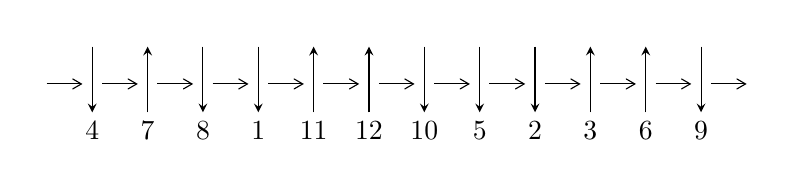
\begin{tikzpicture}[x=20pt, y=17pt]
	% nodes
	\node (C0) at (0, 0) {};
	\node (C1) at (1, 0) {};
	\node (C1U) at (1, +1) {};
	\node (C1D) at (1, -1) {4};

	\node (C2) at (2, 0) {};
	\node (C2U) at (2, +1) {};
	\node (C2D) at (2, -1) {7};

	\node (C3) at (3, 0) {};
	\node (C3U) at (3, +1) {};
	\node (C3D) at (3, -1) {8};

	\node (C4) at (4, 0) {};
	\node (C4U) at (4, +1) {};
	\node (C4D) at (4, -1) {1};

	\node (C5) at (5, 0) {};
	\node (C5U) at (5, +1) {};
	\node (C5D) at (5, -1) {11};

	\node (C6) at (6, 0) {};
	\node (C6U) at (6, +1) {};
	\node (C6D) at (6, -1) {12};

	\node (C7) at (7, 0) {};
	\node (C7U) at (7, +1) {};
	\node (C7D) at (7, -1) {10};

	\node (C8) at (8, 0) {};
	\node (C8U) at (8, +1) {};
	\node (C8D) at (8, -1) {5};

	\node (C9) at (9, 0) {};
	\node (C9U) at (9, +1) {};
	\node (C9D) at (9, -1) {2};

	\node (C10) at (10, 0) {};
	\node (C10U) at (10, +1) {};
	\node (C10D) at (10, -1) {3};

	\node (C11) at (11, 0) {};
	\node (C11U) at (11, +1) {};
	\node (C11D) at (11, -1) {6};

	\node (C12) at (12, 0) {};
	\node (C12U) at (12, +1) {};
	\node (C12D) at (12, -1) {9};
	\node (C13) at (13, 0) {};

	% arrows
	\draw[->,>={angle 60}]
	(C0) edge (C1) (C1) edge (C2) (C2) edge (C3) (C3) edge (C4) (C4) edge (C5) (C5) edge (C6) (C6) edge (C7) (C7) edge (C8) (C8) edge (C9) (C9) edge (C10) (C10) edge (C11) (C11) edge (C12) (C12) edge (C13) ;	\draw[->,>=stealth]
	(C1U) edge (C1D) (C2D) edge (C2U) (C3U) edge (C3D) (C4U) edge (C4D) (C5D) edge (C5U) (C6D) edge (C6U) (C7U) edge (C7D) (C8U) edge (C8D) (C9U) edge (C9D) (C10D) edge (C10U) (C11D) edge (C11U) (C12U) edge (C12D) ;
	\end{tikzpicture} \\
\hhline{~~} \\& 
\textbf{Solving Sequence} \\ \cline{2-2} 
 &
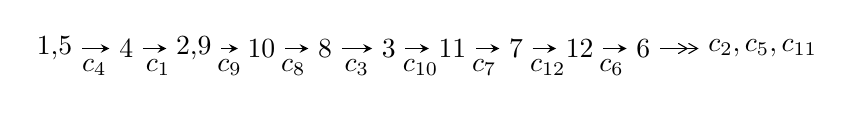
\begin{tikzpicture}[x=23pt, y=7pt]
	% node
	\node (A0) at (-1/8, 0) {1,5};
	\node (A1) at (1, 0) {4};
	\node (A2) at (33/16, 0) {2,9};
	\node (A3) at (25/8, 0) {10};
	\node (A4) at (33/8, 0) {8};
	\node (A5) at (41/8, 0) {3};
	\node (A6) at (49/8, 0) {11};
	\node (A7) at (57/8, 0) {7};
	\node (A8) at (65/8, 0) {12};
	\node (A9) at (73/8, 0) {6};
	\node (C1) at (1/2, -1) {$c_{4}$};
	\node (C2) at (3/2, -1) {$c_{1}$};
	\node (C3) at (21/8, -1) {$c_{9}$};
	\node (C4) at (29/8, -1) {$c_{8}$};
	\node (C5) at (37/8, -1) {$c_{3}$};
	\node (C6) at (45/8, -1) {$c_{10}$};
	\node (C7) at (53/8, -1) {$c_{7}$};
	\node (C8) at (61/8, -1) {$c_{12}$};
	\node (C9) at (69/8, -1) {$c_{6}$};
	\node (A10) at (11, 0) {$c_{2},c_{5},c_{11}$};

	% edge
	\draw[->,>=stealth]	
	(A0) edge (A1) (A1) edge (A2) (A2) edge (A3) (A3) edge (A4) (A4) edge (A5) (A5) edge (A6) (A6) edge (A7) (A7) edge (A8) (A8) edge (A9) ;
	\draw[->>,>={angle 60}]	
	(A9) edge (A10);
\end{tikzpicture} \\ 

\end{tabular} \\

\footnotetext{
The image of knot diagram is generated by the software ``\textbf{Draw programme}" developed by Andrew Bartholomew(\url{http://www.layer8.co.uk/maths/draw/index.htm\#Running-draw}), where we modified some parts for our purpose(\url{https://github.com/CATsTAILs/LinksPainter}).
}\phantom \\ \newline 
\centering \textbf{Ideals for irreducible components\footnotemark of $X_{\text{par}}$} 
 
\begin{align*}
I^u_{1}&=\langle 
-1.16283\times10^{40} u^{55}+2.14434\times10^{41} u^{54}+\cdots+2.38481\times10^{39} b+1.27043\times10^{43},\\
\phantom{I^u_{1}}&\phantom{= \langle  }2.48132\times10^{40} u^{55}-4.23380\times10^{41} u^{54}+\cdots+4.76963\times10^{39} a-6.69755\times10^{42},\\
\phantom{I^u_{1}}&\phantom{= \langle  }u^{56}-18 u^{55}+\cdots-19200 u+1024\rangle \\
I^u_{2}&=\langle 
-3.81235\times10^{34} a^{9} u^{10}+3.02772\times10^{34} a^{8} u^{10}+\cdots-9.29378\times10^{34} a-1.45475\times10^{35},\\
\phantom{I^u_{2}}&\phantom{= \langle  }- u^{10} a^9-5 u^{10} a^8+\cdots-295 a-110,\\
\phantom{I^u_{2}}&\phantom{= \langle  }u^{11}+3 u^{10}+8 u^9+13 u^8+18 u^7+20 u^6+18 u^5+15 u^4+9 u^3+5 u^2+2 u+1\rangle \\
I^u_{3}&=\langle 
2.70992\times10^{15} u^{39}+3.29546\times10^{16} u^{38}+\cdots+1.11311\times10^{15} b-7.54465\times10^{15},\\
\phantom{I^u_{3}}&\phantom{= \langle  }7.54465\times10^{15} u^{39}+1.00790\times10^{17} u^{38}+\cdots+1.11311\times10^{15} a+2.52828\times10^{16},\;u^{40}+13 u^{39}+\cdots+13 u+1\rangle \\
\\
\end{align*}
\raggedright * 3 irreducible components of $\dim_{\mathbb{C}}=0$, with total 206 representations.\\
\footnotetext{All coefficients of polynomials are rational numbers. But the coefficients are sometimes approximated in decimal forms when there is not enough margin.}
\newpage
\renewcommand{\arraystretch}{1}
\centering \section*{I. $I^u_{1}= \langle -1.16\times10^{40} u^{55}+2.14\times10^{41} u^{54}+\cdots+2.38\times10^{39} b+1.27\times10^{43},\;2.48\times10^{40} u^{55}-4.23\times10^{41} u^{54}+\cdots+4.77\times10^{39} a-6.70\times10^{42},\;u^{56}-18 u^{55}+\cdots-19200 u+1024 \rangle$}
\flushleft \textbf{(i) Arc colorings}\\
\begin{tabular}{m{7pt} m{180pt} m{7pt} m{180pt} }
\flushright $a_{1}=$&$\begin{pmatrix}0\\u\end{pmatrix}$ \\
\flushright $a_{5}=$&$\begin{pmatrix}1\\0\end{pmatrix}$ \\
\flushright $a_{4}=$&$\begin{pmatrix}1\\- u^2\end{pmatrix}$ \\
\flushright $a_{2}=$&$\begin{pmatrix}- u\\u^3+u\end{pmatrix}$ \\
\flushright $a_{9}=$&$\begin{pmatrix}-5.20233 u^{55}+88.7659 u^{54}+\cdots-26720.5 u+1404.21\\4.87600 u^{55}-89.9163 u^{54}+\cdots+98480.5 u-5327.19\end{pmatrix}$ \\
\flushright $a_{10}=$&$\begin{pmatrix}-2.55698 u^{55}+46.0061 u^{54}+\cdots-48621.2 u+2671.75\\1.13506 u^{55}-21.4817 u^{54}+\cdots+29846.8 u-1621.76\end{pmatrix}$ \\
\flushright $a_{8}=$&$\begin{pmatrix}-0.326331 u^{55}-1.15037 u^{54}+\cdots+71760.1 u-3922.98\\4.87600 u^{55}-89.9163 u^{54}+\cdots+98480.5 u-5327.19\end{pmatrix}$ \\
\flushright $a_{3}=$&$\begin{pmatrix}-0.799050 u^{55}+16.4891 u^{54}+\cdots-50751.2 u+2785.10\\-0.617890 u^{55}+12.6104 u^{54}+\cdots+508.672 u-185.508\end{pmatrix}$ \\
\flushright $a_{11}=$&$\begin{pmatrix}-1.84666 u^{55}+38.4053 u^{54}+\cdots-114285. u+6283.16\\-2.63618 u^{55}+47.6390 u^{54}+\cdots-48809.0 u+2622.80\end{pmatrix}$ \\
\flushright $a_{7}=$&$\begin{pmatrix}-9.61807 u^{55}+164.399 u^{54}+\cdots-63717.1 u+3382.01\\6.38454 u^{55}-121.688 u^{54}+\cdots+211275. u-11663.2\end{pmatrix}$ \\
\flushright $a_{12}=$&$\begin{pmatrix}-1.22612 u^{55}+17.1359 u^{54}+\cdots+17853.1 u-827.515\\4.93425 u^{55}-84.9272 u^{54}+\cdots+24370.0 u-1255.54\end{pmatrix}$ \\
\flushright $a_{6}=$&$\begin{pmatrix}1.26900 u^{55}-29.2945 u^{54}+\cdots+126784. u-7023.07\\3.92313 u^{55}-71.4238 u^{54}+\cdots+60639.9 u-3214.32\end{pmatrix}$\\&\end{tabular}
\flushleft \textbf{(ii) Obstruction class $= -1$}\\~\\
\flushleft \textbf{(iii) Cusp Shapes $= -24.8470 u^{55}+419.627 u^{54}+\cdots-95591.9 u+4633.30$}\\~\\
\newpage\renewcommand{\arraystretch}{1}
\flushleft \textbf{(iv) u-Polynomials at the component}\newline \\
\begin{tabular}{m{50pt}|m{274pt}}
Crossings & \hspace{64pt}u-Polynomials at each crossing \\
\hline $$\begin{aligned}c_{1},c_{4}\end{aligned}$$&$\begin{aligned}
&u^{56}-18 u^{55}+\cdots-19200 u+1024
\end{aligned}$\\
\hline $$\begin{aligned}c_{2},c_{10}\end{aligned}$$&$\begin{aligned}
&u^{56}-8 u^{54}+\cdots+4 u+1
\end{aligned}$\\
\hline $$\begin{aligned}c_{3},c_{9}\end{aligned}$$&$\begin{aligned}
&u^{56}- u^{55}+\cdots+8 u+1
\end{aligned}$\\
\hline $$\begin{aligned}c_{5},c_{6},c_{11}\end{aligned}$$&$\begin{aligned}
&u^{56}+21 u^{55}+\cdots+4096 u+2048
\end{aligned}$\\
\hline $$\begin{aligned}c_{7}\end{aligned}$$&$\begin{aligned}
&u^{56}-35 u^{55}+\cdots-272 u+32
\end{aligned}$\\
\hline $$\begin{aligned}c_{8},c_{12}\end{aligned}$$&$\begin{aligned}
&u^{56}- u^{55}+\cdots+12 u+1
\end{aligned}$\\
\hline
\end{tabular}\\~\\
\newpage\renewcommand{\arraystretch}{1}
\flushleft \textbf{(v) Riley Polynomials at the component}\newline \\
\begin{tabular}{m{50pt}|m{274pt}}
Crossings & \hspace{64pt}Riley Polynomials at each crossing \\
\hline $$\begin{aligned}c_{1},c_{4}\end{aligned}$$&$\begin{aligned}
&y^{56}+28 y^{55}+\cdots+9502720 y+1048576
\end{aligned}$\\
\hline $$\begin{aligned}c_{2},c_{10}\end{aligned}$$&$\begin{aligned}
&y^{56}-16 y^{55}+\cdots-34 y+1
\end{aligned}$\\
\hline $$\begin{aligned}c_{3},c_{9}\end{aligned}$$&$\begin{aligned}
&y^{56}-7 y^{55}+\cdots-18 y+1
\end{aligned}$\\
\hline $$\begin{aligned}c_{5},c_{6},c_{11}\end{aligned}$$&$\begin{aligned}
&y^{56}-45 y^{55}+\cdots-2097152 y+4194304
\end{aligned}$\\
\hline $$\begin{aligned}c_{7}\end{aligned}$$&$\begin{aligned}
&y^{56}-5 y^{55}+\cdots-9984 y+1024
\end{aligned}$\\
\hline $$\begin{aligned}c_{8},c_{12}\end{aligned}$$&$\begin{aligned}
&y^{56}+33 y^{55}+\cdots+188 y+1
\end{aligned}$\\
\hline
\end{tabular}\\~\\
\newpage\flushleft \textbf{(vi) Complex Volumes and Cusp Shapes}
$$\begin{array}{c|c|c}  
\text{Solutions to }I^u_{1}& \I (\text{vol} + \sqrt{-1}CS) & \text{Cusp shape}\\
 \hline 
\begin{aligned}
u &= -0.020630 + 0.993062 I \\
a &= \phantom{-}1.35474 - 0.80692 I \\
b &= -0.77337 - 1.36199 I\end{aligned}
 & \phantom{-}7.50595 - 4.34710 I & \phantom{-0.000000 } 0 \\ \hline\begin{aligned}
u &= -0.020630 - 0.993062 I \\
a &= \phantom{-}1.35474 + 0.80692 I \\
b &= -0.77337 + 1.36199 I\end{aligned}
 & \phantom{-}7.50595 + 4.34710 I & \phantom{-0.000000 } 0 \\ \hline\begin{aligned}
u &= -0.039442 + 0.978977 I \\
a &= -1.074070 + 0.779942 I \\
b &= \phantom{-}0.721182 + 1.082250 I\end{aligned}
 & \phantom{-}1.92174 - 1.40595 I & \phantom{-0.000000 } 0 \\ \hline\begin{aligned}
u &= -0.039442 - 0.978977 I \\
a &= -1.074070 - 0.779942 I \\
b &= \phantom{-}0.721182 - 1.082250 I\end{aligned}
 & \phantom{-}1.92174 + 1.40595 I & \phantom{-0.000000 } 0 \\ \hline\begin{aligned}
u &= -0.108043 + 1.022290 I \\
a &= \phantom{-}0.803024 - 0.451536 I \\
b &= -0.374842 - 0.869712 I\end{aligned}
 & \phantom{-}2.27427 + 1.77133 I & \phantom{-0.000000 } 0 \\ \hline\begin{aligned}
u &= -0.108043 - 1.022290 I \\
a &= \phantom{-}0.803024 + 0.451536 I \\
b &= -0.374842 + 0.869712 I\end{aligned}
 & \phantom{-}2.27427 - 1.77133 I & \phantom{-0.000000 } 0 \\ \hline\begin{aligned}
u &= \phantom{-}0.308226 + 0.983667 I \\
a &= -0.913578 - 0.497183 I \\
b &= -0.207475 + 1.051900 I\end{aligned}
 & \phantom{-}7.64196 + 4.01513 I & \phantom{-0.000000 } 0 \\ \hline\begin{aligned}
u &= \phantom{-}0.308226 - 0.983667 I \\
a &= -0.913578 + 0.497183 I \\
b &= -0.207475 - 1.051900 I\end{aligned}
 & \phantom{-}7.64196 - 4.01513 I & \phantom{-0.000000 } 0 \\ \hline\begin{aligned}
u &= \phantom{-}0.265198 + 1.021370 I \\
a &= \phantom{-}1.12081 - 0.94691 I \\
b &= -1.26438 - 0.89363 I\end{aligned}
 & \phantom{-}4.37595 - 0.73115 I & \phantom{-0.000000 } 0 \\ \hline\begin{aligned}
u &= \phantom{-}0.265198 - 1.021370 I \\
a &= \phantom{-}1.12081 + 0.94691 I \\
b &= -1.26438 + 0.89363 I\end{aligned}
 & \phantom{-}4.37595 + 0.73115 I & \phantom{-0.000000 } 0\\
 \hline 
 \end{array}$$\newpage$$\begin{array}{c|c|c}  
\text{Solutions to }I^u_{1}& \I (\text{vol} + \sqrt{-1}CS) & \text{Cusp shape}\\
 \hline 
\begin{aligned}
u &= -0.014072 + 1.086320 I \\
a &= -0.985765 + 0.029422 I \\
b &= \phantom{-}0.018090 + 1.071270 I\end{aligned}
 & \phantom{-}7.66190 + 4.32014 I & \phantom{-0.000000 } 0 \\ \hline\begin{aligned}
u &= -0.014072 - 1.086320 I \\
a &= -0.985765 - 0.029422 I \\
b &= \phantom{-}0.018090 - 1.071270 I\end{aligned}
 & \phantom{-}7.66190 - 4.32014 I & \phantom{-0.000000 } 0 \\ \hline\begin{aligned}
u &= \phantom{-}0.865982 + 0.248427 I \\
a &= -0.324727 - 1.231120 I \\
b &= -0.024636 + 1.146800 I\end{aligned}
 & \phantom{-}8.42861 + 2.90333 I & \phantom{-0.000000 } 0 \\ \hline\begin{aligned}
u &= \phantom{-}0.865982 - 0.248427 I \\
a &= -0.324727 + 1.231120 I \\
b &= -0.024636 - 1.146800 I\end{aligned}
 & \phantom{-}8.42861 - 2.90333 I & \phantom{-0.000000 } 0 \\ \hline\begin{aligned}
u &= \phantom{-}1.120500 + 0.105543 I \\
a &= -0.772508 + 0.933095 I \\
b &= \phantom{-}0.964078 - 0.964000 I\end{aligned}
 & \phantom{-}2.4180 + 14.4623 I & \phantom{-0.000000 } 0 \\ \hline\begin{aligned}
u &= \phantom{-}1.120500 - 0.105543 I \\
a &= -0.772508 - 0.933095 I \\
b &= \phantom{-}0.964078 + 0.964000 I\end{aligned}
 & \phantom{-}2.4180 - 14.4623 I & \phantom{-0.000000 } 0 \\ \hline\begin{aligned}
u &= \phantom{-}0.636402 + 0.940838 I \\
a &= \phantom{-}0.832826 + 0.391168 I \\
b &= -0.161987 - 1.032490 I\end{aligned}
 & \phantom{-}1.054820 + 0.344037 I & \phantom{-0.000000 } 0 \\ \hline\begin{aligned}
u &= \phantom{-}0.636402 - 0.940838 I \\
a &= \phantom{-}0.832826 - 0.391168 I \\
b &= -0.161987 + 1.032490 I\end{aligned}
 & \phantom{-}1.054820 - 0.344037 I & \phantom{-0.000000 } 0 \\ \hline\begin{aligned}
u &= -0.707342 + 0.457791 I \\
a &= \phantom{-}0.250539 + 0.339848 I \\
b &= \phantom{-}0.332797 + 0.125694 I\end{aligned}
 & -1.73690 + 0.63011 I & \phantom{-0.000000 } 0 \\ \hline\begin{aligned}
u &= -0.707342 - 0.457791 I \\
a &= \phantom{-}0.250539 - 0.339848 I \\
b &= \phantom{-}0.332797 - 0.125694 I\end{aligned}
 & -1.73690 - 0.63011 I & \phantom{-0.000000 } 0\\
 \hline 
 \end{array}$$\newpage$$\begin{array}{c|c|c}  
\text{Solutions to }I^u_{1}& \I (\text{vol} + \sqrt{-1}CS) & \text{Cusp shape}\\
 \hline 
\begin{aligned}
u &= \phantom{-}1.163670 + 0.137451 I \\
a &= \phantom{-}0.603623 - 0.768644 I \\
b &= -0.808071 + 0.811482 I\end{aligned}
 & -3.35204 + 9.77983 I & \phantom{-0.000000 } 0 \\ \hline\begin{aligned}
u &= \phantom{-}1.163670 - 0.137451 I \\
a &= \phantom{-}0.603623 + 0.768644 I \\
b &= -0.808071 - 0.811482 I\end{aligned}
 & -3.35204 - 9.77983 I & \phantom{-0.000000 } 0 \\ \hline\begin{aligned}
u &= \phantom{-}0.786118 + 0.200802 I \\
a &= \phantom{-}0.79806 - 1.39804 I \\
b &= -0.908100 + 0.938770 I\end{aligned}
 & \phantom{-}3.66238 + 7.09364 I & \phantom{-0.000000 } 0 \\ \hline\begin{aligned}
u &= \phantom{-}0.786118 - 0.200802 I \\
a &= \phantom{-}0.79806 + 1.39804 I \\
b &= -0.908100 - 0.938770 I\end{aligned}
 & \phantom{-}3.66238 - 7.09364 I & \phantom{-0.000000 } 0 \\ \hline\begin{aligned}
u &= \phantom{-}0.508543 + 1.110890 I \\
a &= -1.41993 + 0.31079 I \\
b &= \phantom{-}1.06734 + 1.41934 I\end{aligned}
 & \phantom{-}0.83845 - 6.82264 I & \phantom{-0.000000 } 0 \\ \hline\begin{aligned}
u &= \phantom{-}0.508543 - 1.110890 I \\
a &= -1.41993 - 0.31079 I \\
b &= \phantom{-}1.06734 - 1.41934 I\end{aligned}
 & \phantom{-}0.83845 + 6.82264 I & \phantom{-0.000000 } 0 \\ \hline\begin{aligned}
u &= \phantom{-}1.197390 + 0.249700 I \\
a &= -0.296015 + 0.680603 I \\
b &= \phantom{-}0.524393 - 0.741036 I\end{aligned}
 & -1.42857 + 4.12269 I & \phantom{-0.000000 } 0 \\ \hline\begin{aligned}
u &= \phantom{-}1.197390 - 0.249700 I \\
a &= -0.296015 - 0.680603 I \\
b &= \phantom{-}0.524393 + 0.741036 I\end{aligned}
 & -1.42857 - 4.12269 I & \phantom{-0.000000 } 0 \\ \hline\begin{aligned}
u &= -0.731646 + 0.982650 I \\
a &= \phantom{-}0.071450 - 0.268151 I \\
b &= -0.211222 - 0.266402 I\end{aligned}
 & -0.20428 + 4.86627 I & \phantom{-0.000000 } 0 \\ \hline\begin{aligned}
u &= -0.731646 - 0.982650 I \\
a &= \phantom{-}0.071450 + 0.268151 I \\
b &= -0.211222 + 0.266402 I\end{aligned}
 & -0.20428 - 4.86627 I & \phantom{-0.000000 } 0\\
 \hline 
 \end{array}$$\newpage$$\begin{array}{c|c|c}  
\text{Solutions to }I^u_{1}& \I (\text{vol} + \sqrt{-1}CS) & \text{Cusp shape}\\
 \hline 
\begin{aligned}
u &= \phantom{-}0.669015 + 1.080040 I \\
a &= -0.911259 - 0.400202 I \\
b &= \phantom{-}0.177414 + 1.251930 I\end{aligned}
 & \phantom{-}1.76632 - 5.80202 I & \phantom{-0.000000 } 0 \\ \hline\begin{aligned}
u &= \phantom{-}0.669015 - 1.080040 I \\
a &= -0.911259 + 0.400202 I \\
b &= \phantom{-}0.177414 - 1.251930 I\end{aligned}
 & \phantom{-}1.76632 + 5.80202 I & \phantom{-0.000000 } 0 \\ \hline\begin{aligned}
u &= \phantom{-}0.625036 + 0.353244 I \\
a &= -0.54480 + 1.54547 I \\
b &= \phantom{-}0.886448 - 0.773523 I\end{aligned}
 & -1.39205 + 2.34242 I & \phantom{-0.000000 } 0 \\ \hline\begin{aligned}
u &= \phantom{-}0.625036 - 0.353244 I \\
a &= -0.54480 - 1.54547 I \\
b &= \phantom{-}0.886448 + 0.773523 I\end{aligned}
 & -1.39205 - 2.34242 I & \phantom{-0.000000 } 0 \\ \hline\begin{aligned}
u &= \phantom{-}0.505060 + 1.184110 I \\
a &= \phantom{-}1.35790 - 0.41395 I \\
b &= -1.17598 - 1.39883 I\end{aligned}
 & \phantom{-}6.61152 - 11.89410 I & \phantom{-0.000000 } 0 \\ \hline\begin{aligned}
u &= \phantom{-}0.505060 - 1.184110 I \\
a &= \phantom{-}1.35790 + 0.41395 I \\
b &= -1.17598 + 1.39883 I\end{aligned}
 & \phantom{-}6.61152 + 11.89410 I & \phantom{-0.000000 } 0 \\ \hline\begin{aligned}
u &= \phantom{-}0.182497 + 1.304990 I \\
a &= \phantom{-}0.644331 - 0.308225 I \\
b &= -0.519818 - 0.784595 I\end{aligned}
 & \phantom{-}5.19823 - 0.38486 I & \phantom{-0.000000 } 0 \\ \hline\begin{aligned}
u &= \phantom{-}0.182497 - 1.304990 I \\
a &= \phantom{-}0.644331 + 0.308225 I \\
b &= -0.519818 + 0.784595 I\end{aligned}
 & \phantom{-}5.19823 + 0.38486 I & \phantom{-0.000000 } 0 \\ \hline\begin{aligned}
u &= \phantom{-}0.355367 + 1.286890 I \\
a &= -1.096520 + 0.095012 I \\
b &= \phantom{-}0.51194 + 1.37734 I\end{aligned}
 & \phantom{-}13.11000 - 1.19025 I & \phantom{-0.000000 } 0 \\ \hline\begin{aligned}
u &= \phantom{-}0.355367 - 1.286890 I \\
a &= -1.096520 - 0.095012 I \\
b &= \phantom{-}0.51194 - 1.37734 I\end{aligned}
 & \phantom{-}13.11000 + 1.19025 I & \phantom{-0.000000 } 0\\
 \hline 
 \end{array}$$\newpage$$\begin{array}{c|c|c}  
\text{Solutions to }I^u_{1}& \I (\text{vol} + \sqrt{-1}CS) & \text{Cusp shape}\\
 \hline 
\begin{aligned}
u &= \phantom{-}0.598285 + 1.230550 I \\
a &= \phantom{-}1.107960 + 0.185777 I \\
b &= -0.43427 - 1.47455 I\end{aligned}
 & \phantom{-}11.31360 - 8.41411 I & \phantom{-0.000000 } 0 \\ \hline\begin{aligned}
u &= \phantom{-}0.598285 - 1.230550 I \\
a &= \phantom{-}1.107960 - 0.185777 I \\
b &= -0.43427 + 1.47455 I\end{aligned}
 & \phantom{-}11.31360 + 8.41411 I & \phantom{-0.000000 } 0 \\ \hline\begin{aligned}
u &= \phantom{-}0.58111 + 1.32533 I \\
a &= -1.200120 + 0.346172 I \\
b &= \phantom{-}1.15620 + 1.38939 I\end{aligned}
 & \phantom{-}6.2353 - 20.4547 I & \phantom{-0.000000 } 0 \\ \hline\begin{aligned}
u &= \phantom{-}0.58111 - 1.32533 I \\
a &= -1.200120 - 0.346172 I \\
b &= \phantom{-}1.15620 - 1.38939 I\end{aligned}
 & \phantom{-}6.2353 + 20.4547 I & \phantom{-0.000000 } 0 \\ \hline\begin{aligned}
u &= \phantom{-}0.62767 + 1.30970 I \\
a &= -0.994170 + 0.135205 I \\
b &= \phantom{-}0.80109 + 1.21720 I\end{aligned}
 & \phantom{-}2.00380 - 10.50370 I & \phantom{-0.000000 } 0 \\ \hline\begin{aligned}
u &= \phantom{-}0.62767 - 1.30970 I \\
a &= -0.994170 - 0.135205 I \\
b &= \phantom{-}0.80109 - 1.21720 I\end{aligned}
 & \phantom{-}2.00380 + 10.50370 I & \phantom{-0.000000 } 0 \\ \hline\begin{aligned}
u &= \phantom{-}0.59880 + 1.32640 I \\
a &= \phantom{-}1.086980 - 0.284336 I \\
b &= -1.02803 - 1.27151 I\end{aligned}
 & \phantom{-}0.3961 - 15.9494 I & \phantom{-0.000000 } 0 \\ \hline\begin{aligned}
u &= \phantom{-}0.59880 - 1.32640 I \\
a &= \phantom{-}1.086980 + 0.284336 I \\
b &= -1.02803 + 1.27151 I\end{aligned}
 & \phantom{-}0.3961 + 15.9494 I & \phantom{-0.000000 } 0 \\ \hline\begin{aligned}
u &= \phantom{-}0.22066 + 1.55593 I \\
a &= -0.375610 - 0.024297 I \\
b &= \phantom{-}0.045077 + 0.589783 I\end{aligned}
 & \phantom{-}2.64603 + 4.04647 I & \phantom{-0.000000 } 0 \\ \hline\begin{aligned}
u &= \phantom{-}0.22066 - 1.55593 I \\
a &= -0.375610 + 0.024297 I \\
b &= \phantom{-}0.045077 - 0.589783 I\end{aligned}
 & \phantom{-}2.64603 - 4.04647 I & \phantom{-0.000000 } 0\\
 \hline 
 \end{array}$$\newpage$$\begin{array}{c|c|c}  
\text{Solutions to }I^u_{1}& \I (\text{vol} + \sqrt{-1}CS) & \text{Cusp shape}\\
 \hline 
\begin{aligned}
u &= \phantom{-}0.38904 + 1.53423 I \\
a &= \phantom{-}0.396798 + 0.277446 I \\
b &= \phantom{-}0.271294 - 0.716716 I\end{aligned}
 & \phantom{-}7.74841 + 8.71344 I & \phantom{-0.000000 } 0 \\ \hline\begin{aligned}
u &= \phantom{-}0.38904 - 1.53423 I \\
a &= \phantom{-}0.396798 - 0.277446 I \\
b &= \phantom{-}0.271294 + 0.716716 I\end{aligned}
 & \phantom{-}7.74841 - 8.71344 I & \phantom{-0.000000 } 0 \\ \hline\begin{aligned}
u &= \phantom{-}0.257267 + 0.289166 I \\
a &= \phantom{-}1.44997 + 0.86456 I \\
b &= -0.123028 - 0.641707 I\end{aligned}
 & \phantom{-}1.02800 + 1.00373 I & \phantom{-}4.20772 - 2.96757 I \\ \hline\begin{aligned}
u &= \phantom{-}0.257267 - 0.289166 I \\
a &= \phantom{-}1.44997 - 0.86456 I \\
b &= -0.123028 + 0.641707 I\end{aligned}
 & \phantom{-}1.02800 - 1.00373 I & \phantom{-}4.20772 + 2.96757 I \\ \hline\begin{aligned}
u &= -1.84068 + 0.56528 I \\
a &= \phantom{-}0.0300490 - 0.0308640 I \\
b &= \phantom{-}0.0378637 - 0.0737969 I\end{aligned}
 & -3.96631 + 2.95414 I & \phantom{-0.000000 } 0 \\ \hline\begin{aligned}
u &= -1.84068 - 0.56528 I \\
a &= \phantom{-}0.0300490 + 0.0308640 I \\
b &= \phantom{-}0.0378637 + 0.0737969 I\end{aligned}
 & -3.96631 - 2.95414 I & \phantom{-0.000000 } 0\\
 \hline 
 \end{array}$$\newpage\newpage\renewcommand{\arraystretch}{1}
\centering \section*{II. $I^u_{2}= \langle -3.81\times10^{34} a^{9} u^{10}+3.03\times10^{34} a^{8} u^{10}+\cdots-9.29\times10^{34} a-1.45\times10^{35},\;- u^{10} a^9-5 u^{10} a^8+\cdots-295 a-110,\;u^{11}+3 u^{10}+\cdots+2 u+1 \rangle$}
\flushleft \textbf{(i) Arc colorings}\\
\begin{tabular}{m{7pt} m{180pt} m{7pt} m{180pt} }
\flushright $a_{1}=$&$\begin{pmatrix}0\\u\end{pmatrix}$ \\
\flushright $a_{5}=$&$\begin{pmatrix}1\\0\end{pmatrix}$ \\
\flushright $a_{4}=$&$\begin{pmatrix}1\\- u^2\end{pmatrix}$ \\
\flushright $a_{2}=$&$\begin{pmatrix}- u\\u^3+u\end{pmatrix}$ \\
\flushright $a_{9}=$&$\begin{pmatrix}a\\0.907182 a^{9} u^{10}-0.720474 a^{8} u^{10}+\cdots+2.21154 a+3.46170\end{pmatrix}$ \\
\flushright $a_{10}=$&$\begin{pmatrix}-0.492257 a^{9} u^{10}+0.00342511 a^{8} u^{10}+\cdots+1.48128 a-0.271791\\-4.10347 a^{9} u^{10}+2.09816 a^{8} u^{10}+\cdots+2.51299 a+1.85463\end{pmatrix}$ \\
\flushright $a_{8}=$&$\begin{pmatrix}0.907182 a^{9} u^{10}-0.720474 a^{8} u^{10}+\cdots+3.21154 a+3.46170\\0.907182 a^{9} u^{10}-0.720474 a^{8} u^{10}+\cdots+2.21154 a+3.46170\end{pmatrix}$ \\
\flushright $a_{3}=$&$\begin{pmatrix}5.07518 a^{9} u^{10}+1.03594 a^{8} u^{10}+\cdots-5.93466 a+1.08613\\3.75966 a^{9} u^{10}+0.538146 a^{8} u^{10}+\cdots-2.76372 a-0.0156369\end{pmatrix}$ \\
\flushright $a_{11}=$&$\begin{pmatrix}1.84368 a^{9} u^{10}-0.176828 a^{8} u^{10}+\cdots-7.34564 a-5.54919\\3.36159 a^{9} u^{10}-0.793945 a^{8} u^{10}+\cdots-1.68096 a-0.279916\end{pmatrix}$ \\
\flushright $a_{7}=$&$\begin{pmatrix}1.78885 a^{9} u^{10}-1.21260 a^{8} u^{10}+\cdots+2.00706 a+4.05887\\-0.457991 a^{9} u^{10}+0.204668 a^{8} u^{10}+\cdots-2.09454 a+0.327920\end{pmatrix}$ \\
\flushright $a_{12}=$&$\begin{pmatrix}a^2 u\\1.80869 a^{9} u^{10}+0.558889 a^{8} u^{10}+\cdots+0.709045 a-0.353266\end{pmatrix}$ \\
\flushright $a_{6}=$&$\begin{pmatrix}2.93332 a^{9} u^{10}-1.13790 a^{8} u^{10}+\cdots-1.40440 a+2.91248\\3.28932 a^{9} u^{10}-0.643942 a^{8} u^{10}+\cdots+0.763603 a+2.90564\end{pmatrix}$\\&\end{tabular}
\flushleft \textbf{(ii) Obstruction class $= -1$}\\~\\
\flushleft \textbf{(iii) Cusp Shapes $= -6.21162 a^{9} u^{10}+5.41134 a^{8} u^{10}+\cdots+9.56003 a-2.29340$}\\~\\
\newpage\renewcommand{\arraystretch}{1}
\flushleft \textbf{(iv) u-Polynomials at the component}\newline \\
\begin{tabular}{m{50pt}|m{274pt}}
Crossings & \hspace{64pt}u-Polynomials at each crossing \\
\hline $$\begin{aligned}c_{1},c_{4}\end{aligned}$$&$\begin{aligned}
&(u^{11}+3 u^{10}+\cdots+2 u+1)^{10}
\end{aligned}$\\
\hline $$\begin{aligned}c_{2},c_{10}\end{aligned}$$&$\begin{aligned}
&u^{110}+3 u^{109}+\cdots-72 u+1
\end{aligned}$\\
\hline $$\begin{aligned}c_{3},c_{9}\end{aligned}$$&$\begin{aligned}
&u^{110}+u^{109}+\cdots-288500 u-72659
\end{aligned}$\\
\hline $$\begin{aligned}c_{5},c_{6},c_{11}\end{aligned}$$&$\begin{aligned}
&(u^5- u^4-2 u^3+u^2+u+1)^{22}
\end{aligned}$\\
\hline $$\begin{aligned}c_{7}\end{aligned}$$&$\begin{aligned}
&(u^{11}+5 u^{10}+12 u^9+15 u^8+8 u^7-4 u^6-8 u^5-3 u^4+3 u^3+3 u^2-1)^{10}
\end{aligned}$\\
\hline $$\begin{aligned}c_{8},c_{12}\end{aligned}$$&$\begin{aligned}
&u^{110}- u^{109}+\cdots+26520 u-547
\end{aligned}$\\
\hline
\end{tabular}\\~\\
\newpage\renewcommand{\arraystretch}{1}
\flushleft \textbf{(v) Riley Polynomials at the component}\newline \\
\begin{tabular}{m{50pt}|m{274pt}}
Crossings & \hspace{64pt}Riley Polynomials at each crossing \\
\hline $$\begin{aligned}c_{1},c_{4}\end{aligned}$$&$\begin{aligned}
&(y^{11}+7 y^{10}+\cdots-6 y-1)^{10}
\end{aligned}$\\
\hline $$\begin{aligned}c_{2},c_{10}\end{aligned}$$&$\begin{aligned}
&y^{110}+35 y^{109}+\cdots-7528 y+1
\end{aligned}$\\
\hline $$\begin{aligned}c_{3},c_{9}\end{aligned}$$&$\begin{aligned}
&y^{110}-25 y^{109}+\cdots+621106657840 y+5279330281
\end{aligned}$\\
\hline $$\begin{aligned}c_{5},c_{6},c_{11}\end{aligned}$$&$\begin{aligned}
&(y^5-5 y^4+8 y^3-3 y^2- y-1)^{22}
\end{aligned}$\\
\hline $$\begin{aligned}c_{7}\end{aligned}$$&$\begin{aligned}
&(y^{11}- y^{10}+\cdots+6 y-1)^{10}
\end{aligned}$\\
\hline $$\begin{aligned}c_{8},c_{12}\end{aligned}$$&$\begin{aligned}
&y^{110}-21 y^{109}+\cdots-39626548 y+299209
\end{aligned}$\\
\hline
\end{tabular}\\~\\
\newpage\flushleft \textbf{(vi) Complex Volumes and Cusp Shapes}
$$\begin{array}{c|c|c}  
\text{Solutions to }I^u_{2}& \I (\text{vol} + \sqrt{-1}CS) & \text{Cusp shape}\\
 \hline 
\begin{aligned}
u &= \phantom{-}0.253759 + 0.946686 I \\
a &= -1.214280 + 0.254968 I \\
b &= \phantom{-}1.406490 - 0.038889 I\end{aligned}
 & -1.17818 - 3.68571 I & -3.92092 + 4.58213 I \\ \hline\begin{aligned}
u &= \phantom{-}0.253759 + 0.946686 I \\
a &= \phantom{-}1.00777 - 0.99699 I \\
b &= -1.66471 - 0.72815 I\end{aligned}
 & \phantom{-}4.36528 - 0.81546 I & \phantom{-}0.30828 + 5.51419 I \\ \hline\begin{aligned}
u &= \phantom{-}0.253759 + 0.946686 I \\
a &= -0.33322 + 1.39637 I \\
b &= \phantom{-}0.549509 + 1.084840 I\end{aligned}
 & -1.17818 - 3.68571 I & -3.92092 + 4.58213 I \\ \hline\begin{aligned}
u &= \phantom{-}0.253759 + 0.946686 I \\
a &= -0.278887 + 0.480235 I \\
b &= \phantom{-}2.56562 - 0.97418 I\end{aligned}
 & \phantom{-}4.36528 - 9.61712 I & \phantom{-}0.30828 + 12.51136 I \\ \hline\begin{aligned}
u &= \phantom{-}0.253759 + 0.946686 I \\
a &= \phantom{-}0.127850 - 0.489290 I \\
b &= \phantom{-}0.68642 - 1.90567 I\end{aligned}
 & \phantom{-}0.89380 - 5.21629 I & -2.95489 + 9.01278 I \\ \hline\begin{aligned}
u &= \phantom{-}0.253759 + 0.946686 I \\
a &= \phantom{-}0.405552 - 0.162342 I \\
b &= -1.86813 + 0.97949 I\end{aligned}
 & -1.17818 - 6.74687 I & -3.92092 + 13.44342 I \\ \hline\begin{aligned}
u &= \phantom{-}0.253759 + 0.946686 I \\
a &= \phantom{-}1.15735 - 1.44823 I \\
b &= -1.199570 - 0.701047 I\end{aligned}
 & \phantom{-}4.36528 - 0.81546 I & \phantom{-}0.30828 + 5.51419 I \\ \hline\begin{aligned}
u &= \phantom{-}0.253759 + 0.946686 I \\
a &= \phantom{-}1.69672 + 1.17989 I \\
b &= -0.495647 + 0.003128 I\end{aligned}
 & \phantom{-}0.89380 - 5.21629 I & -2.95489 + 9.01278 I \\ \hline\begin{aligned}
u &= \phantom{-}0.253759 + 0.946686 I \\
a &= -0.47180 - 2.09980 I \\
b &= -0.256599 - 0.342734 I\end{aligned}
 & -1.17818 - 6.74687 I & -3.92092 + 13.44342 I \\ \hline\begin{aligned}
u &= \phantom{-}0.253759 + 0.946686 I \\
a &= \phantom{-}0.28232 + 2.78578 I \\
b &= \phantom{-}0.525402 + 0.142154 I\end{aligned}
 & \phantom{-}4.36528 - 9.61712 I & \phantom{-}0.30828 + 12.51136 I\\
 \hline 
 \end{array}$$\newpage$$\begin{array}{c|c|c}  
\text{Solutions to }I^u_{2}& \I (\text{vol} + \sqrt{-1}CS) & \text{Cusp shape}\\
 \hline 
\begin{aligned}
u &= \phantom{-}0.253759 - 0.946686 I \\
a &= -1.214280 - 0.254968 I \\
b &= \phantom{-}1.406490 + 0.038889 I\end{aligned}
 & -1.17818 + 3.68571 I & -3.92092 - 4.58213 I \\ \hline\begin{aligned}
u &= \phantom{-}0.253759 - 0.946686 I \\
a &= \phantom{-}1.00777 + 0.99699 I \\
b &= -1.66471 + 0.72815 I\end{aligned}
 & \phantom{-}4.36528 + 0.81546 I & \phantom{-}0.30828 - 5.51419 I \\ \hline\begin{aligned}
u &= \phantom{-}0.253759 - 0.946686 I \\
a &= -0.33322 - 1.39637 I \\
b &= \phantom{-}0.549509 - 1.084840 I\end{aligned}
 & -1.17818 + 3.68571 I & -3.92092 - 4.58213 I \\ \hline\begin{aligned}
u &= \phantom{-}0.253759 - 0.946686 I \\
a &= -0.278887 - 0.480235 I \\
b &= \phantom{-}2.56562 + 0.97418 I\end{aligned}
 & \phantom{-}4.36528 + 9.61712 I & \phantom{-}0.30828 - 12.51136 I \\ \hline\begin{aligned}
u &= \phantom{-}0.253759 - 0.946686 I \\
a &= \phantom{-}0.127850 + 0.489290 I \\
b &= \phantom{-}0.68642 + 1.90567 I\end{aligned}
 & \phantom{-}0.89380 + 5.21629 I & -2.95489 - 9.01278 I \\ \hline\begin{aligned}
u &= \phantom{-}0.253759 - 0.946686 I \\
a &= \phantom{-}0.405552 + 0.162342 I \\
b &= -1.86813 - 0.97949 I\end{aligned}
 & -1.17818 + 6.74687 I & -3.92092 - 13.44342 I \\ \hline\begin{aligned}
u &= \phantom{-}0.253759 - 0.946686 I \\
a &= \phantom{-}1.15735 + 1.44823 I \\
b &= -1.199570 + 0.701047 I\end{aligned}
 & \phantom{-}4.36528 + 0.81546 I & \phantom{-}0.30828 - 5.51419 I \\ \hline\begin{aligned}
u &= \phantom{-}0.253759 - 0.946686 I \\
a &= \phantom{-}1.69672 - 1.17989 I \\
b &= -0.495647 - 0.003128 I\end{aligned}
 & \phantom{-}0.89380 + 5.21629 I & -2.95489 - 9.01278 I \\ \hline\begin{aligned}
u &= \phantom{-}0.253759 - 0.946686 I \\
a &= -0.47180 + 2.09980 I \\
b &= -0.256599 + 0.342734 I\end{aligned}
 & -1.17818 + 6.74687 I & -3.92092 - 13.44342 I \\ \hline\begin{aligned}
u &= \phantom{-}0.253759 - 0.946686 I \\
a &= \phantom{-}0.28232 - 2.78578 I \\
b &= \phantom{-}0.525402 - 0.142154 I\end{aligned}
 & \phantom{-}4.36528 + 9.61712 I & \phantom{-}0.30828 - 12.51136 I\\
 \hline 
 \end{array}$$\newpage$$\begin{array}{c|c|c}  
\text{Solutions to }I^u_{2}& \I (\text{vol} + \sqrt{-1}CS) & \text{Cusp shape}\\
 \hline 
\begin{aligned}
u &= -1.10821\phantom{ +0.000000I} \\
a &= \phantom{-}1.06944\phantom{ +0.000000I} \\
b &= -1.43122\phantom{ +0.000000I}\end{aligned}
 & -1.62261\phantom{ +0.000000I} & -14.7800\phantom{ +0.000000I} \\ \hline\begin{aligned}
u &= -1.10821\phantom{ +0.000000I} \\
a &= \phantom{-}0.780503 + 0.437504 I \\
b &= -0.756153 - 0.220972 I\end{aligned}
 & -3.69459 - 1.53058 I & -15.7462 + 4.4306 I \\ \hline\begin{aligned}
u &= -1.10821\phantom{ +0.000000I} \\
a &= \phantom{-}0.780503 - 0.437504 I \\
b &= -0.756153 + 0.220972 I\end{aligned}
 & -3.69459 + 1.53058 I & -15.7462 - 4.4306 I \\ \hline\begin{aligned}
u &= -1.10821\phantom{ +0.000000I} \\
a &= -0.696511 + 0.898164 I \\
b &= \phantom{-}0.625664 - 0.610265 I\end{aligned}
 & \phantom{-}1.84887 + 4.40083 I & -11.51702 - 3.49859 I \\ \hline\begin{aligned}
u &= -1.10821\phantom{ +0.000000I} \\
a &= -0.696511 - 0.898164 I \\
b &= \phantom{-}0.625664 + 0.610265 I\end{aligned}
 & \phantom{-}1.84887 - 4.40083 I & -11.51702 + 3.49859 I \\ \hline\begin{aligned}
u &= -1.10821\phantom{ +0.000000I} \\
a &= \phantom{-}0.564570 + 0.550675 I \\
b &= -0.771883 - 0.995357 I\end{aligned}
 & \phantom{-}1.84887 - 4.40083 I & -11.51702 + 3.49859 I \\ \hline\begin{aligned}
u &= -1.10821\phantom{ +0.000000I} \\
a &= \phantom{-}0.564570 - 0.550675 I \\
b &= -0.771883 + 0.995357 I\end{aligned}
 & \phantom{-}1.84887 + 4.40083 I & -11.51702 - 3.49859 I \\ \hline\begin{aligned}
u &= -1.10821\phantom{ +0.000000I} \\
a &= -0.682318 + 0.199395 I \\
b &= \phantom{-}0.864963 - 0.484847 I\end{aligned}
 & -3.69459 + 1.53058 I & -15.7462 - 4.4306 I \\ \hline\begin{aligned}
u &= -1.10821\phantom{ +0.000000I} \\
a &= -0.682318 - 0.199395 I \\
b &= \phantom{-}0.864963 + 0.484847 I\end{aligned}
 & -3.69459 - 1.53058 I & -15.7462 + 4.4306 I \\ \hline\begin{aligned}
u &= -1.10821\phantom{ +0.000000I} \\
a &= -1.29147\phantom{ +0.000000I} \\
b &= \phantom{-}1.18517\phantom{ +0.000000I}\end{aligned}
 & -1.62261\phantom{ +0.000000I} & -14.7800\phantom{ +0.000000I}\\
 \hline 
 \end{array}$$\newpage$$\begin{array}{c|c|c}  
\text{Solutions to }I^u_{2}& \I (\text{vol} + \sqrt{-1}CS) & \text{Cusp shape}\\
 \hline 
\begin{aligned}
u &= -0.572881 + 0.536287 I \\
a &= \phantom{-}0.516653 + 0.935169 I \\
b &= -0.0210317 - 0.0200933 I\end{aligned}
 & -1.73984 + 0.71721 I & -7.12070 - 0.63295 I \\ \hline\begin{aligned}
u &= -0.572881 + 0.536287 I \\
a &= \phantom{-}0.845678 + 0.745623 I \\
b &= -1.32964 + 0.56677 I\end{aligned}
 & \phantom{-}0.33215 + 2.24779 I & -6.15467 - 5.06360 I \\ \hline\begin{aligned}
u &= -0.572881 + 0.536287 I \\
a &= -1.111270 - 0.406619 I \\
b &= \phantom{-}0.472061 - 1.079550 I\end{aligned}
 & -1.73984 + 3.77836 I & -7.12070 - 9.49424 I \\ \hline\begin{aligned}
u &= -0.572881 + 0.536287 I \\
a &= -0.588376 + 0.498556 I \\
b &= -1.04070 - 0.97694 I\end{aligned}
 & \phantom{-}3.80363 - 2.15305 I & -2.89150 - 1.56501 I \\ \hline\begin{aligned}
u &= -0.572881 + 0.536287 I \\
a &= \phantom{-}1.348260 + 0.235231 I \\
b &= -0.31739 + 1.60636 I\end{aligned}
 & \phantom{-}3.80363 + 6.64862 I & -2.89150 - 8.56218 I \\ \hline\begin{aligned}
u &= -0.572881 + 0.536287 I \\
a &= \phantom{-}1.37932 - 0.59320 I \\
b &= -0.854688 + 0.363014 I\end{aligned}
 & -1.73984 + 3.77836 I & -7.12070 - 9.49424 I \\ \hline\begin{aligned}
u &= -0.572881 + 0.536287 I \\
a &= -0.11737 - 1.81518 I \\
b &= -0.069700 + 0.601152 I\end{aligned}
 & \phantom{-}3.80363 - 2.15305 I & -2.89150 - 1.56501 I \\ \hline\begin{aligned}
u &= -0.572881 + 0.536287 I \\
a &= -1.73057 - 0.63068 I \\
b &= \phantom{-}0.884341 - 0.026373 I\end{aligned}
 & \phantom{-}0.33215 + 2.24779 I & -6.15467 - 5.06360 I \\ \hline\begin{aligned}
u &= -0.572881 + 0.536287 I \\
a &= -0.0020671 - 0.0370092 I \\
b &= \phantom{-}0.797500 + 0.258666 I\end{aligned}
 & -1.73984 + 0.71721 I & -7.12070 - 0.63295 I \\ \hline\begin{aligned}
u &= -0.572881 + 0.536287 I \\
a &= -1.69422 + 1.21800 I \\
b &= \phantom{-}0.898542 - 0.588293 I\end{aligned}
 & \phantom{-}3.80363 + 6.64862 I & -2.89150 - 8.56218 I\\
 \hline 
 \end{array}$$\newpage$$\begin{array}{c|c|c}  
\text{Solutions to }I^u_{2}& \I (\text{vol} + \sqrt{-1}CS) & \text{Cusp shape}\\
 \hline 
\begin{aligned}
u &= -0.572881 - 0.536287 I \\
a &= \phantom{-}0.516653 - 0.935169 I \\
b &= -0.0210317 + 0.0200933 I\end{aligned}
 & -1.73984 - 0.71721 I & -7.12070 + 0.63295 I \\ \hline\begin{aligned}
u &= -0.572881 - 0.536287 I \\
a &= \phantom{-}0.845678 - 0.745623 I \\
b &= -1.32964 - 0.56677 I\end{aligned}
 & \phantom{-}0.33215 - 2.24779 I & -6.15467 + 5.06360 I \\ \hline\begin{aligned}
u &= -0.572881 - 0.536287 I \\
a &= -1.111270 + 0.406619 I \\
b &= \phantom{-}0.472061 + 1.079550 I\end{aligned}
 & -1.73984 - 3.77836 I & -7.12070 + 9.49424 I \\ \hline\begin{aligned}
u &= -0.572881 - 0.536287 I \\
a &= -0.588376 - 0.498556 I \\
b &= -1.04070 + 0.97694 I\end{aligned}
 & \phantom{-}3.80363 + 2.15305 I & -2.89150 + 1.56501 I \\ \hline\begin{aligned}
u &= -0.572881 - 0.536287 I \\
a &= \phantom{-}1.348260 - 0.235231 I \\
b &= -0.31739 - 1.60636 I\end{aligned}
 & \phantom{-}3.80363 - 6.64862 I & -2.89150 + 8.56218 I \\ \hline\begin{aligned}
u &= -0.572881 - 0.536287 I \\
a &= \phantom{-}1.37932 + 0.59320 I \\
b &= -0.854688 - 0.363014 I\end{aligned}
 & -1.73984 - 3.77836 I & -7.12070 + 9.49424 I \\ \hline\begin{aligned}
u &= -0.572881 - 0.536287 I \\
a &= -0.11737 + 1.81518 I \\
b &= -0.069700 - 0.601152 I\end{aligned}
 & \phantom{-}3.80363 + 2.15305 I & -2.89150 + 1.56501 I \\ \hline\begin{aligned}
u &= -0.572881 - 0.536287 I \\
a &= -1.73057 + 0.63068 I \\
b &= \phantom{-}0.884341 + 0.026373 I\end{aligned}
 & \phantom{-}0.33215 - 2.24779 I & -6.15467 + 5.06360 I \\ \hline\begin{aligned}
u &= -0.572881 - 0.536287 I \\
a &= -0.0020671 + 0.0370092 I \\
b &= \phantom{-}0.797500 - 0.258666 I\end{aligned}
 & -1.73984 - 0.71721 I & -7.12070 + 0.63295 I \\ \hline\begin{aligned}
u &= -0.572881 - 0.536287 I \\
a &= -1.69422 - 1.21800 I \\
b &= \phantom{-}0.898542 + 0.588293 I\end{aligned}
 & \phantom{-}3.80363 - 6.64862 I & -2.89150 + 8.56218 I\\
 \hline 
 \end{array}$$\newpage$$\begin{array}{c|c|c}  
\text{Solutions to }I^u_{2}& \I (\text{vol} + \sqrt{-1}CS) & \text{Cusp shape}\\
 \hline 
\begin{aligned}
u &= -0.290349 + 1.272230 I \\
a &= \phantom{-}1.016900 + 0.255279 I \\
b &= -0.375763 + 0.413196 I\end{aligned}
 & \phantom{-}3.31489 + 3.47016 I & \phantom{-}4.35571 - 1.79686 I \\ \hline\begin{aligned}
u &= -0.290349 + 1.272230 I \\
a &= \phantom{-}0.454399 + 0.971570 I \\
b &= -0.805599 + 0.755681 I\end{aligned}
 & \phantom{-}5.38688 + 5.00074 I & \phantom{-}5.32173 - 6.22751 I \\ \hline\begin{aligned}
u &= -0.290349 + 1.272230 I \\
a &= -0.850343 - 0.184422 I \\
b &= \phantom{-}1.53517 - 1.63532 I\end{aligned}
 & \phantom{-}8.85836 + 9.40157 I & \phantom{-}8.58490 - 9.72610 I \\ \hline\begin{aligned}
u &= -0.290349 + 1.272230 I \\
a &= -0.701934 - 0.473022 I \\
b &= \phantom{-}1.368000 - 0.296006 I\end{aligned}
 & \phantom{-}5.38688 + 5.00074 I & \phantom{-}5.32173 - 6.22751 I \\ \hline\begin{aligned}
u &= -0.290349 + 1.272230 I \\
a &= \phantom{-}0.725998 + 0.291082 I \\
b &= -1.32280 + 1.23898 I\end{aligned}
 & \phantom{-}3.31489 + 6.53132 I & \phantom{-}4.35571 - 10.65816 I \\ \hline\begin{aligned}
u &= -0.290349 + 1.272230 I \\
a &= -1.335750 + 0.013724 I \\
b &= -0.014845 - 0.550001 I\end{aligned}
 & \phantom{-}8.85836 + 0.59990 I & \phantom{-}8.58490 - 2.72893 I \\ \hline\begin{aligned}
u &= -0.290349 + 1.272230 I \\
a &= -1.151200 - 0.777020 I \\
b &= \phantom{-}0.581117 - 0.839123 I\end{aligned}
 & \phantom{-}3.31489 + 6.53132 I & \phantom{-}4.35571 - 10.65816 I \\ \hline\begin{aligned}
u &= -0.290349 + 1.272230 I \\
a &= -0.372772 - 0.210283 I \\
b &= \phantom{-}0.620030 - 1.219620 I\end{aligned}
 & \phantom{-}3.31489 + 3.47016 I & \phantom{-}4.35571 - 1.79686 I \\ \hline\begin{aligned}
u &= -0.290349 + 1.272230 I \\
a &= \phantom{-}0.408379 - 0.104869 I \\
b &= -0.37038 + 1.70337 I\end{aligned}
 & \phantom{-}8.85836 + 0.59990 I & \phantom{-}8.58490 - 2.72893 I \\ \hline\begin{aligned}
u &= -0.290349 + 1.272230 I \\
a &= \phantom{-}1.48352 + 0.86811 I \\
b &= -0.481525 + 1.028290 I\end{aligned}
 & \phantom{-}8.85836 + 9.40157 I & \phantom{-}8.58490 - 9.72610 I\\
 \hline 
 \end{array}$$\newpage$$\begin{array}{c|c|c}  
\text{Solutions to }I^u_{2}& \I (\text{vol} + \sqrt{-1}CS) & \text{Cusp shape}\\
 \hline 
\begin{aligned}
u &= -0.290349 - 1.272230 I \\
a &= \phantom{-}1.016900 - 0.255279 I \\
b &= -0.375763 - 0.413196 I\end{aligned}
 & \phantom{-}3.31489 - 3.47016 I & \phantom{-}4.35571 + 1.79686 I \\ \hline\begin{aligned}
u &= -0.290349 - 1.272230 I \\
a &= \phantom{-}0.454399 - 0.971570 I \\
b &= -0.805599 - 0.755681 I\end{aligned}
 & \phantom{-}5.38688 - 5.00074 I & \phantom{-}5.32173 + 6.22751 I \\ \hline\begin{aligned}
u &= -0.290349 - 1.272230 I \\
a &= -0.850343 + 0.184422 I \\
b &= \phantom{-}1.53517 + 1.63532 I\end{aligned}
 & \phantom{-}8.85836 - 9.40157 I & \phantom{-}8.58490 + 9.72610 I \\ \hline\begin{aligned}
u &= -0.290349 - 1.272230 I \\
a &= -0.701934 + 0.473022 I \\
b &= \phantom{-}1.368000 + 0.296006 I\end{aligned}
 & \phantom{-}5.38688 - 5.00074 I & \phantom{-}5.32173 + 6.22751 I \\ \hline\begin{aligned}
u &= -0.290349 - 1.272230 I \\
a &= \phantom{-}0.725998 - 0.291082 I \\
b &= -1.32280 - 1.23898 I\end{aligned}
 & \phantom{-}3.31489 - 6.53132 I & \phantom{-}4.35571 + 10.65816 I \\ \hline\begin{aligned}
u &= -0.290349 - 1.272230 I \\
a &= -1.335750 - 0.013724 I \\
b &= -0.014845 + 0.550001 I\end{aligned}
 & \phantom{-}8.85836 - 0.59990 I & \phantom{-}8.58490 + 2.72893 I \\ \hline\begin{aligned}
u &= -0.290349 - 1.272230 I \\
a &= -1.151200 + 0.777020 I \\
b &= \phantom{-}0.581117 + 0.839123 I\end{aligned}
 & \phantom{-}3.31489 - 6.53132 I & \phantom{-}4.35571 + 10.65816 I \\ \hline\begin{aligned}
u &= -0.290349 - 1.272230 I \\
a &= -0.372772 + 0.210283 I \\
b &= \phantom{-}0.620030 + 1.219620 I\end{aligned}
 & \phantom{-}3.31489 - 3.47016 I & \phantom{-}4.35571 + 1.79686 I \\ \hline\begin{aligned}
u &= -0.290349 - 1.272230 I \\
a &= \phantom{-}0.408379 + 0.104869 I \\
b &= -0.37038 - 1.70337 I\end{aligned}
 & \phantom{-}8.85836 - 0.59990 I & \phantom{-}8.58490 + 2.72893 I \\ \hline\begin{aligned}
u &= -0.290349 - 1.272230 I \\
a &= \phantom{-}1.48352 - 0.86811 I \\
b &= -0.481525 - 1.028290 I\end{aligned}
 & \phantom{-}8.85836 - 9.40157 I & \phantom{-}8.58490 + 9.72610 I\\
 \hline 
 \end{array}$$\newpage$$\begin{array}{c|c|c}  
\text{Solutions to }I^u_{2}& \I (\text{vol} + \sqrt{-1}CS) & \text{Cusp shape}\\
 \hline 
\begin{aligned}
u &= \phantom{-}0.234018 + 0.605151 I \\
a &= -0.699171 + 0.624862 I \\
b &= \phantom{-}1.199470 - 0.525523 I\end{aligned}
 & -2.11873 + 1.17383 I & -6.95250 + 4.51398 I \\ \hline\begin{aligned}
u &= \phantom{-}0.234018 + 0.605151 I \\
a &= -0.252370 + 0.599876 I \\
b &= -0.79612 + 1.45703 I\end{aligned}
 & -0.04675 + 2.70441 I & -5.98648 + 0.08333 I \\ \hline\begin{aligned}
u &= \phantom{-}0.234018 + 0.605151 I \\
a &= \phantom{-}0.04344 - 1.46541 I \\
b &= -1.62502 - 0.02887 I\end{aligned}
 & \phantom{-}3.42473 - 1.69642 I & -2.72331 + 3.58191 I \\ \hline\begin{aligned}
u &= \phantom{-}0.234018 + 0.605151 I \\
a &= \phantom{-}0.14061 - 1.54546 I \\
b &= -0.442259 - 1.327510 I\end{aligned}
 & -2.11873 + 4.23499 I & -6.95250 - 4.34732 I \\ \hline\begin{aligned}
u &= \phantom{-}0.234018 + 0.605151 I \\
a &= -0.29345 + 1.76062 I \\
b &= \phantom{-}0.94330 + 1.69305 I\end{aligned}
 & \phantom{-}3.42473 + 7.10524 I & -2.72331 - 3.41526 I \\ \hline\begin{aligned}
u &= \phantom{-}0.234018 + 0.605151 I \\
a &= \phantom{-}0.08866 + 2.01639 I \\
b &= \phantom{-}0.541754 + 0.276875 I\end{aligned}
 & -2.11873 + 1.17383 I & -6.95250 + 4.51398 I \\ \hline\begin{aligned}
u &= \phantom{-}0.234018 + 0.605151 I \\
a &= \phantom{-}2.15416 + 0.10221 I \\
b &= -0.968141 + 0.276574 I\end{aligned}
 & -2.11873 + 4.23499 I & -6.95250 - 4.34732 I \\ \hline\begin{aligned}
u &= \phantom{-}0.234018 + 0.605151 I \\
a &= \phantom{-}0.94485 - 2.31993 I \\
b &= -0.896960 + 0.316647 I\end{aligned}
 & \phantom{-}3.42473 - 1.69642 I & -2.72331 + 3.58191 I \\ \hline\begin{aligned}
u &= \phantom{-}0.234018 + 0.605151 I \\
a &= -1.65193 - 1.95440 I \\
b &= \phantom{-}0.422074 + 0.012340 I\end{aligned}
 & -0.04675 + 2.70441 I & -5.98648 + 0.08333 I \\ \hline\begin{aligned}
u &= \phantom{-}0.234018 + 0.605151 I \\
a &= -2.95816 + 0.41484 I \\
b &= \phantom{-}1.134110 - 0.234436 I\end{aligned}
 & \phantom{-}3.42473 + 7.10524 I & -2.72331 - 3.41526 I\\
 \hline 
 \end{array}$$\newpage$$\begin{array}{c|c|c}  
\text{Solutions to }I^u_{2}& \I (\text{vol} + \sqrt{-1}CS) & \text{Cusp shape}\\
 \hline 
\begin{aligned}
u &= \phantom{-}0.234018 - 0.605151 I \\
a &= -0.699171 - 0.624862 I \\
b &= \phantom{-}1.199470 + 0.525523 I\end{aligned}
 & -2.11873 - 1.17383 I & -6.95250 - 4.51398 I \\ \hline\begin{aligned}
u &= \phantom{-}0.234018 - 0.605151 I \\
a &= -0.252370 - 0.599876 I \\
b &= -0.79612 - 1.45703 I\end{aligned}
 & -0.04675 - 2.70441 I & -5.98648 - 0.08333 I \\ \hline\begin{aligned}
u &= \phantom{-}0.234018 - 0.605151 I \\
a &= \phantom{-}0.04344 + 1.46541 I \\
b &= -1.62502 + 0.02887 I\end{aligned}
 & \phantom{-}3.42473 + 1.69642 I & -2.72331 - 3.58191 I \\ \hline\begin{aligned}
u &= \phantom{-}0.234018 - 0.605151 I \\
a &= \phantom{-}0.14061 + 1.54546 I \\
b &= -0.442259 + 1.327510 I\end{aligned}
 & -2.11873 - 4.23499 I & -6.95250 + 4.34732 I \\ \hline\begin{aligned}
u &= \phantom{-}0.234018 - 0.605151 I \\
a &= -0.29345 - 1.76062 I \\
b &= \phantom{-}0.94330 - 1.69305 I\end{aligned}
 & \phantom{-}3.42473 - 7.10524 I & -2.72331 + 3.41526 I \\ \hline\begin{aligned}
u &= \phantom{-}0.234018 - 0.605151 I \\
a &= \phantom{-}0.08866 - 2.01639 I \\
b &= \phantom{-}0.541754 - 0.276875 I\end{aligned}
 & -2.11873 - 1.17383 I & -6.95250 - 4.51398 I \\ \hline\begin{aligned}
u &= \phantom{-}0.234018 - 0.605151 I \\
a &= \phantom{-}2.15416 - 0.10221 I \\
b &= -0.968141 - 0.276574 I\end{aligned}
 & -2.11873 - 4.23499 I & -6.95250 + 4.34732 I \\ \hline\begin{aligned}
u &= \phantom{-}0.234018 - 0.605151 I \\
a &= \phantom{-}0.94485 + 2.31993 I \\
b &= -0.896960 - 0.316647 I\end{aligned}
 & \phantom{-}3.42473 + 1.69642 I & -2.72331 - 3.58191 I \\ \hline\begin{aligned}
u &= \phantom{-}0.234018 - 0.605151 I \\
a &= -1.65193 + 1.95440 I \\
b &= \phantom{-}0.422074 - 0.012340 I\end{aligned}
 & -0.04675 - 2.70441 I & -5.98648 - 0.08333 I \\ \hline\begin{aligned}
u &= \phantom{-}0.234018 - 0.605151 I \\
a &= -2.95816 - 0.41484 I \\
b &= \phantom{-}1.134110 + 0.234436 I\end{aligned}
 & \phantom{-}3.42473 - 7.10524 I & -2.72331 + 3.41526 I\\
 \hline 
 \end{array}$$\newpage$$\begin{array}{c|c|c}  
\text{Solutions to }I^u_{2}& \I (\text{vol} + \sqrt{-1}CS) & \text{Cusp shape}\\
 \hline 
\begin{aligned}
u &= -0.57044 + 1.34258 I \\
a &= -0.785939 - 0.641440 I \\
b &= \phantom{-}1.115300 - 0.438195 I\end{aligned}
 & \phantom{-}2.51638 + 5.92443 I & -5.68931 - 10.02355 I \\ \hline\begin{aligned}
u &= -0.57044 + 1.34258 I \\
a &= \phantom{-}0.946446 + 0.248467 I \\
b &= -1.056870 + 0.809620 I\end{aligned}
 & \phantom{-}0.44440 + 7.45501 I & -6.6553 - 14.4542 I \\ \hline\begin{aligned}
u &= -0.57044 + 1.34258 I \\
a &= \phantom{-}0.941032 + 0.405944 I \\
b &= -0.80426 + 1.48503 I\end{aligned}
 & \phantom{-}5.98786 + 10.32530 I & -2.42614 - 13.52213 I \\ \hline\begin{aligned}
u &= -0.57044 + 1.34258 I \\
a &= -0.794135 - 0.449777 I \\
b &= \phantom{-}0.87348 - 1.12895 I\end{aligned}
 & \phantom{-}0.44440 + 7.45501 I & -6.6553 - 14.4542 I \\ \hline\begin{aligned}
u &= -0.57044 + 1.34258 I \\
a &= -1.152550 - 0.109335 I \\
b &= \phantom{-}1.08182 - 1.03185 I\end{aligned}
 & \phantom{-}5.98786 + 10.32530 I & -2.42614 - 13.52213 I \\ \hline\begin{aligned}
u &= -0.57044 + 1.34258 I \\
a &= \phantom{-}0.575454 + 0.586211 I \\
b &= -1.30952 + 0.68928 I\end{aligned}
 & \phantom{-}2.51638 + 5.92443 I & -5.68931 - 10.02355 I \\ \hline\begin{aligned}
u &= -0.57044 + 1.34258 I \\
a &= \phantom{-}0.568427 + 0.363833 I \\
b &= -0.457563 + 0.652864 I\end{aligned}
 & \phantom{-}0.44440 + 4.39385 I & -6.65534 - 5.59290 I \\ \hline\begin{aligned}
u &= -0.57044 + 1.34258 I \\
a &= \phantom{-}0.513603 - 0.308604 I \\
b &= -0.387048 + 0.710839 I\end{aligned}
 & \phantom{-}5.98786 + 1.52359 I & -2.42614 - 6.52496 I \\ \hline\begin{aligned}
u &= -0.57044 + 1.34258 I \\
a &= -0.552249 - 0.053645 I \\
b &= -0.121346 - 0.865594 I\end{aligned}
 & \phantom{-}5.98786 + 1.52359 I & -2.42614 - 6.52496 I \\ \hline\begin{aligned}
u &= -0.57044 + 1.34258 I \\
a &= -0.534574 - 0.113677 I \\
b &= \phantom{-}0.812729 - 0.555614 I\end{aligned}
 & \phantom{-}0.44440 + 4.39385 I & -6.65534 - 5.59290 I\\
 \hline 
 \end{array}$$\newpage$$\begin{array}{c|c|c}  
\text{Solutions to }I^u_{2}& \I (\text{vol} + \sqrt{-1}CS) & \text{Cusp shape}\\
 \hline 
\begin{aligned}
u &= -0.57044 - 1.34258 I \\
a &= -0.785939 + 0.641440 I \\
b &= \phantom{-}1.115300 + 0.438195 I\end{aligned}
 & \phantom{-}2.51638 - 5.92443 I & -5.68931 + 10.02355 I \\ \hline\begin{aligned}
u &= -0.57044 - 1.34258 I \\
a &= \phantom{-}0.946446 - 0.248467 I \\
b &= -1.056870 - 0.809620 I\end{aligned}
 & \phantom{-}0.44440 - 7.45501 I & -6.6553 + 14.4542 I \\ \hline\begin{aligned}
u &= -0.57044 - 1.34258 I \\
a &= \phantom{-}0.941032 - 0.405944 I \\
b &= -0.80426 - 1.48503 I\end{aligned}
 & \phantom{-}5.98786 - 10.32530 I & -2.42614 + 13.52213 I \\ \hline\begin{aligned}
u &= -0.57044 - 1.34258 I \\
a &= -0.794135 + 0.449777 I \\
b &= \phantom{-}0.87348 + 1.12895 I\end{aligned}
 & \phantom{-}0.44440 - 7.45501 I & -6.6553 + 14.4542 I \\ \hline\begin{aligned}
u &= -0.57044 - 1.34258 I \\
a &= -1.152550 + 0.109335 I \\
b &= \phantom{-}1.08182 + 1.03185 I\end{aligned}
 & \phantom{-}5.98786 - 10.32530 I & -2.42614 + 13.52213 I \\ \hline\begin{aligned}
u &= -0.57044 - 1.34258 I \\
a &= \phantom{-}0.575454 - 0.586211 I \\
b &= -1.30952 - 0.68928 I\end{aligned}
 & \phantom{-}2.51638 - 5.92443 I & -5.68931 + 10.02355 I \\ \hline\begin{aligned}
u &= -0.57044 - 1.34258 I \\
a &= \phantom{-}0.568427 - 0.363833 I \\
b &= -0.457563 - 0.652864 I\end{aligned}
 & \phantom{-}0.44440 - 4.39385 I & -6.65534 + 5.59290 I \\ \hline\begin{aligned}
u &= -0.57044 - 1.34258 I \\
a &= \phantom{-}0.513603 + 0.308604 I \\
b &= -0.387048 - 0.710839 I\end{aligned}
 & \phantom{-}5.98786 - 1.52359 I & -2.42614 + 6.52496 I \\ \hline\begin{aligned}
u &= -0.57044 - 1.34258 I \\
a &= -0.552249 + 0.053645 I \\
b &= -0.121346 + 0.865594 I\end{aligned}
 & \phantom{-}5.98786 - 1.52359 I & -2.42614 + 6.52496 I \\ \hline\begin{aligned}
u &= -0.57044 - 1.34258 I \\
a &= -0.534574 + 0.113677 I \\
b &= \phantom{-}0.812729 + 0.555614 I\end{aligned}
 & \phantom{-}0.44440 - 4.39385 I & -6.65534 + 5.59290 I\\
 \hline 
 \end{array}$$\newpage\newpage\renewcommand{\arraystretch}{1}
\centering \section*{III. $I^u_{3}= \langle 2.71\times10^{15} u^{39}+3.30\times10^{16} u^{38}+\cdots+1.11\times10^{15} b-7.54\times10^{15},\;7.54\times10^{15} u^{39}+1.01\times10^{17} u^{38}+\cdots+1.11\times10^{15} a+2.53\times10^{16},\;u^{40}+13 u^{39}+\cdots+13 u+1 \rangle$}
\flushleft \textbf{(i) Arc colorings}\\
\begin{tabular}{m{7pt} m{180pt} m{7pt} m{180pt} }
\flushright $a_{1}=$&$\begin{pmatrix}0\\u\end{pmatrix}$ \\
\flushright $a_{5}=$&$\begin{pmatrix}1\\0\end{pmatrix}$ \\
\flushright $a_{4}=$&$\begin{pmatrix}1\\- u^2\end{pmatrix}$ \\
\flushright $a_{2}=$&$\begin{pmatrix}- u\\u^3+u\end{pmatrix}$ \\
\flushright $a_{9}=$&$\begin{pmatrix}-6.77798 u^{39}-90.5483 u^{38}+\cdots-212.235 u-22.7137\\-2.43455 u^{39}-29.6058 u^{38}+\cdots+65.4001 u+6.77798\end{pmatrix}$ \\
\flushright $a_{10}=$&$\begin{pmatrix}-10.2563 u^{39}-134.947 u^{38}+\cdots-192.304 u-20.6290\\-1.84869 u^{39}-22.1837 u^{38}+\cdots+52.6431 u+5.51276\end{pmatrix}$ \\
\flushright $a_{8}=$&$\begin{pmatrix}-9.21253 u^{39}-120.154 u^{38}+\cdots-146.835 u-15.9357\\-2.43455 u^{39}-29.6058 u^{38}+\cdots+65.4001 u+6.77798\end{pmatrix}$ \\
\flushright $a_{3}=$&$\begin{pmatrix}3.74877 u^{39}+42.7879 u^{38}+\cdots+38.4646 u+7.38528\\-3.49534 u^{39}-47.8903 u^{38}+\cdots-80.5441 u-7.24412\end{pmatrix}$ \\
\flushright $a_{11}=$&$\begin{pmatrix}-0.531367 u^{39}-10.4633 u^{38}+\cdots-324.781 u-29.9644\\0.254134 u^{39}-0.214753 u^{38}+\cdots-26.7084 u-0.649031\end{pmatrix}$ \\
\flushright $a_{7}=$&$\begin{pmatrix}8.31931 u^{39}+104.042 u^{38}+\cdots+177.914 u+13.1129\\-4.40001 u^{39}-59.1809 u^{38}+\cdots-87.4335 u-6.88478\end{pmatrix}$ \\
\flushright $a_{12}=$&$\begin{pmatrix}-7.95615 u^{39}-103.494 u^{38}+\cdots-209.573 u-21.6492\\-0.0636530 u^{39}-0.0518015 u^{38}+\cdots+82.7808 u+7.95615\end{pmatrix}$ \\
\flushright $a_{6}=$&$\begin{pmatrix}3.73312 u^{39}+51.5946 u^{38}+\cdots+156.225 u+11.4603\\-0.745671 u^{39}-9.45596 u^{38}+\cdots-33.4183 u-2.55272\end{pmatrix}$\\&\end{tabular}
\flushleft \textbf{(ii) Obstruction class $= 1$}\\~\\
\flushleft \textbf{(iii) Cusp Shapes $= \frac{49209887514998933}{1113111866454425} u^{39}+\frac{663479598064214632}{1113111866454425} u^{38}+\cdots+\frac{1082356982452410238}{1113111866454425} u+\frac{83103687073235062}{1113111866454425}$}\\~\\
\newpage\renewcommand{\arraystretch}{1}
\flushleft \textbf{(iv) u-Polynomials at the component}\newline \\
\begin{tabular}{m{50pt}|m{274pt}}
Crossings & \hspace{64pt}u-Polynomials at each crossing \\
\hline $$\begin{aligned}c_{1}\end{aligned}$$&$\begin{aligned}
&u^{40}-13 u^{39}+\cdots-13 u+1
\end{aligned}$\\
\hline $$\begin{aligned}c_{2},c_{10}\end{aligned}$$&$\begin{aligned}
&u^{40}+11 u^{38}+\cdots-5 u-1
\end{aligned}$\\
\hline $$\begin{aligned}c_{3},c_{9}\end{aligned}$$&$\begin{aligned}
&u^{40}- u^{39}+\cdots+13 u-7
\end{aligned}$\\
\hline $$\begin{aligned}c_{4}\end{aligned}$$&$\begin{aligned}
&u^{40}+13 u^{39}+\cdots+13 u+1
\end{aligned}$\\
\hline $$\begin{aligned}c_{5},c_{6}\end{aligned}$$&$\begin{aligned}
&u^{40}+2 u^{39}+\cdots-3 u+1
\end{aligned}$\\
\hline $$\begin{aligned}c_{7}\end{aligned}$$&$\begin{aligned}
&u^{40}-22 u^{39}+\cdots-7 u+1
\end{aligned}$\\
\hline $$\begin{aligned}c_{8},c_{12}\end{aligned}$$&$\begin{aligned}
&u^{40}-3 u^{39}+\cdots-7 u-1
\end{aligned}$\\
\hline $$\begin{aligned}c_{11}\end{aligned}$$&$\begin{aligned}
&u^{40}-2 u^{39}+\cdots+3 u+1
\end{aligned}$\\
\hline
\end{tabular}\\~\\
\newpage\renewcommand{\arraystretch}{1}
\flushleft \textbf{(v) Riley Polynomials at the component}\newline \\
\begin{tabular}{m{50pt}|m{274pt}}
Crossings & \hspace{64pt}Riley Polynomials at each crossing \\
\hline $$\begin{aligned}c_{1},c_{4}\end{aligned}$$&$\begin{aligned}
&y^{40}+21 y^{39}+\cdots+y+1
\end{aligned}$\\
\hline $$\begin{aligned}c_{2},c_{10}\end{aligned}$$&$\begin{aligned}
&y^{40}+22 y^{39}+\cdots-5 y+1
\end{aligned}$\\
\hline $$\begin{aligned}c_{3},c_{9}\end{aligned}$$&$\begin{aligned}
&y^{40}-13 y^{39}+\cdots+223 y+49
\end{aligned}$\\
\hline $$\begin{aligned}c_{5},c_{6},c_{11}\end{aligned}$$&$\begin{aligned}
&y^{40}-40 y^{39}+\cdots+y+1
\end{aligned}$\\
\hline $$\begin{aligned}c_{7}\end{aligned}$$&$\begin{aligned}
&y^{40}-4 y^{39}+\cdots-17 y+1
\end{aligned}$\\
\hline $$\begin{aligned}c_{8},c_{12}\end{aligned}$$&$\begin{aligned}
&y^{40}-13 y^{39}+\cdots+5 y+1
\end{aligned}$\\
\hline
\end{tabular}\\~\\
\newpage\flushleft \textbf{(vi) Complex Volumes and Cusp Shapes}
$$\begin{array}{c|c|c}  
\text{Solutions to }I^u_{3}& \I (\text{vol} + \sqrt{-1}CS) & \text{Cusp shape}\\
 \hline 
\begin{aligned}
u &= -0.302193 + 0.961756 I \\
a &= \phantom{-}1.36527 + 1.24156 I \\
b &= -1.60665 + 0.93787 I\end{aligned}
 & \phantom{-}4.66350 + 0.68253 I & \phantom{-0.000000 } 0 \\ \hline\begin{aligned}
u &= -0.302193 - 0.961756 I \\
a &= \phantom{-}1.36527 - 1.24156 I \\
b &= -1.60665 - 0.93787 I\end{aligned}
 & \phantom{-}4.66350 - 0.68253 I & \phantom{-0.000000 } 0 \\ \hline\begin{aligned}
u &= \phantom{-}0.179612 + 1.004620 I \\
a &= -0.962397 - 0.715529 I \\
b &= \phantom{-}0.545979 - 1.095360 I\end{aligned}
 & \phantom{-}1.59926 - 4.62320 I & \phantom{-0.000000 } 0 \\ \hline\begin{aligned}
u &= \phantom{-}0.179612 - 1.004620 I \\
a &= -0.962397 + 0.715529 I \\
b &= \phantom{-}0.545979 + 1.095360 I\end{aligned}
 & \phantom{-}1.59926 + 4.62320 I & \phantom{-0.000000 } 0 \\ \hline\begin{aligned}
u &= -0.958542 + 0.081933 I \\
a &= \phantom{-}0.753873 - 0.799079 I \\
b &= -0.657149 + 0.827718 I\end{aligned}
 & \phantom{-}2.62062 + 4.54167 I & \phantom{-0.000000 } 0 \\ \hline\begin{aligned}
u &= -0.958542 - 0.081933 I \\
a &= \phantom{-}0.753873 + 0.799079 I \\
b &= -0.657149 - 0.827718 I\end{aligned}
 & \phantom{-}2.62062 - 4.54167 I & \phantom{-0.000000 } 0 \\ \hline\begin{aligned}
u &= \phantom{-}0.475218 + 0.832257 I \\
a &= \phantom{-}0.105588 + 0.652587 I \\
b &= -0.492943 + 0.397997 I\end{aligned}
 & -1.07028 - 6.02780 I & \phantom{-0.000000 } 0 \\ \hline\begin{aligned}
u &= \phantom{-}0.475218 - 0.832257 I \\
a &= \phantom{-}0.105588 - 0.652587 I \\
b &= -0.492943 - 0.397997 I\end{aligned}
 & -1.07028 + 6.02780 I & \phantom{-0.000000 } 0 \\ \hline\begin{aligned}
u &= -1.04794\phantom{ +0.000000I} \\
a &= \phantom{-}1.25425\phantom{ +0.000000I} \\
b &= -1.31438\phantom{ +0.000000I}\end{aligned}
 & -1.05586\phantom{ +0.000000I} & \phantom{-0.000000 } 0 \\ \hline\begin{aligned}
u &= \phantom{-}0.198993 + 0.857079 I \\
a &= \phantom{-}0.529987 + 1.135620 I \\
b &= -0.867850 + 0.680220 I\end{aligned}
 & -1.29856 - 5.76607 I & -4.50377 + 5.05173 I\\
 \hline 
 \end{array}$$\newpage$$\begin{array}{c|c|c}  
\text{Solutions to }I^u_{3}& \I (\text{vol} + \sqrt{-1}CS) & \text{Cusp shape}\\
 \hline 
\begin{aligned}
u &= \phantom{-}0.198993 - 0.857079 I \\
a &= \phantom{-}0.529987 - 1.135620 I \\
b &= -0.867850 - 0.680220 I\end{aligned}
 & -1.29856 + 5.76607 I & -4.50377 - 5.05173 I \\ \hline\begin{aligned}
u &= \phantom{-}0.074658 + 0.859654 I \\
a &= -0.68878 - 1.60477 I \\
b &= \phantom{-}1.32812 - 0.71192 I\end{aligned}
 & \phantom{-}4.46569 - 8.28143 I & \phantom{-}3.21081 + 5.41950 I \\ \hline\begin{aligned}
u &= \phantom{-}0.074658 - 0.859654 I \\
a &= -0.68878 + 1.60477 I \\
b &= \phantom{-}1.32812 + 0.71192 I\end{aligned}
 & \phantom{-}4.46569 + 8.28143 I & \phantom{-}3.21081 - 5.41950 I \\ \hline\begin{aligned}
u &= -0.283043 + 0.807141 I \\
a &= \phantom{-}0.52662 + 1.64564 I \\
b &= -1.47732 - 0.04073 I\end{aligned}
 & \phantom{-}4.14697 + 1.84028 I & \phantom{-}11.6326 - 8.8001 I \\ \hline\begin{aligned}
u &= -0.283043 - 0.807141 I \\
a &= \phantom{-}0.52662 - 1.64564 I \\
b &= -1.47732 + 0.04073 I\end{aligned}
 & \phantom{-}4.14697 - 1.84028 I & \phantom{-}11.6326 + 8.8001 I \\ \hline\begin{aligned}
u &= -1.17611\phantom{ +0.000000I} \\
a &= -0.765486\phantom{ +0.000000I} \\
b &= \phantom{-}0.900298\phantom{ +0.000000I}\end{aligned}
 & -3.35566\phantom{ +0.000000I} & \phantom{-0.000000 } 0 \\ \hline\begin{aligned}
u &= \phantom{-}0.129149 + 0.793883 I \\
a &= \phantom{-}1.202550 + 0.737313 I \\
b &= -0.430032 + 1.049900 I\end{aligned}
 & \phantom{-}0.81760 + 3.07351 I & \phantom{-}4.23417 - 3.39461 I \\ \hline\begin{aligned}
u &= \phantom{-}0.129149 - 0.793883 I \\
a &= \phantom{-}1.202550 - 0.737313 I \\
b &= -0.430032 - 1.049900 I\end{aligned}
 & \phantom{-}0.81760 - 3.07351 I & \phantom{-}4.23417 + 3.39461 I \\ \hline\begin{aligned}
u &= -0.058694 + 1.270490 I \\
a &= -0.112190 - 0.771707 I \\
b &= \phantom{-}0.987030 - 0.097241 I\end{aligned}
 & \phantom{-}6.17011 + 7.94112 I & \phantom{-0.000000 } 0 \\ \hline\begin{aligned}
u &= -0.058694 - 1.270490 I \\
a &= -0.112190 + 0.771707 I \\
b &= \phantom{-}0.987030 + 0.097241 I\end{aligned}
 & \phantom{-}6.17011 - 7.94112 I & \phantom{-0.000000 } 0\\
 \hline 
 \end{array}$$\newpage$$\begin{array}{c|c|c}  
\text{Solutions to }I^u_{3}& \I (\text{vol} + \sqrt{-1}CS) & \text{Cusp shape}\\
 \hline 
\begin{aligned}
u &= -0.528320 + 1.195220 I \\
a &= -1.074290 - 0.258592 I \\
b &= \phantom{-}0.87664 - 1.14739 I\end{aligned}
 & \phantom{-}1.00109 + 6.32670 I & \phantom{-0.000000 } 0 \\ \hline\begin{aligned}
u &= -0.528320 - 1.195220 I \\
a &= -1.074290 + 0.258592 I \\
b &= \phantom{-}0.87664 + 1.14739 I\end{aligned}
 & \phantom{-}1.00109 - 6.32670 I & \phantom{-0.000000 } 0 \\ \hline\begin{aligned}
u &= -0.489235 + 1.291200 I \\
a &= \phantom{-}1.114280 + 0.317822 I \\
b &= -0.95552 + 1.28328 I\end{aligned}
 & \phantom{-}6.72770 + 9.59494 I & \phantom{-0.000000 } 0 \\ \hline\begin{aligned}
u &= -0.489235 - 1.291200 I \\
a &= \phantom{-}1.114280 - 0.317822 I \\
b &= -0.95552 - 1.28328 I\end{aligned}
 & \phantom{-}6.72770 - 9.59494 I & \phantom{-0.000000 } 0 \\ \hline\begin{aligned}
u &= \phantom{-}0.477512 + 0.363096 I \\
a &= \phantom{-}0.170665 - 0.915354 I \\
b &= \phantom{-}0.413856 - 0.375125 I\end{aligned}
 & -2.02197 + 2.31681 I & -7.44581 - 1.97781 I \\ \hline\begin{aligned}
u &= \phantom{-}0.477512 - 0.363096 I \\
a &= \phantom{-}0.170665 + 0.915354 I \\
b &= \phantom{-}0.413856 + 0.375125 I\end{aligned}
 & -2.02197 - 2.31681 I & -7.44581 + 1.97781 I \\ \hline\begin{aligned}
u &= -0.372659 + 0.418740 I \\
a &= -1.60084 - 0.62809 I \\
b &= \phantom{-}0.859573 - 0.436271 I\end{aligned}
 & -2.23378 + 2.17048 I & -9.45805 - 4.37787 I \\ \hline\begin{aligned}
u &= -0.372659 - 0.418740 I \\
a &= -1.60084 + 0.62809 I \\
b &= \phantom{-}0.859573 + 0.436271 I\end{aligned}
 & -2.23378 - 2.17048 I & -9.45805 + 4.37787 I \\ \hline\begin{aligned}
u &= -0.53269 + 1.34734 I \\
a &= \phantom{-}0.688381 + 0.653576 I \\
b &= -1.247280 + 0.579327 I\end{aligned}
 & \phantom{-}3.13515 + 5.60962 I & \phantom{-0.000000 } 0 \\ \hline\begin{aligned}
u &= -0.53269 - 1.34734 I \\
a &= \phantom{-}0.688381 - 0.653576 I \\
b &= -1.247280 - 0.579327 I\end{aligned}
 & \phantom{-}3.13515 - 5.60962 I & \phantom{-0.000000 } 0\\
 \hline 
 \end{array}$$\newpage$$\begin{array}{c|c|c}  
\text{Solutions to }I^u_{3}& \I (\text{vol} + \sqrt{-1}CS) & \text{Cusp shape}\\
 \hline 
\begin{aligned}
u &= -0.61009 + 1.31777 I \\
a &= -0.717459 - 0.307067 I \\
b &= \phantom{-}0.842360 - 0.758103 I\end{aligned}
 & \phantom{-}0.65588 + 6.25816 I & \phantom{-0.000000 } 0 \\ \hline\begin{aligned}
u &= -0.61009 - 1.31777 I \\
a &= -0.717459 + 0.307067 I \\
b &= \phantom{-}0.842360 + 0.758103 I\end{aligned}
 & \phantom{-}0.65588 - 6.25816 I & \phantom{-0.000000 } 0 \\ \hline\begin{aligned}
u &= -0.23388 + 1.45246 I \\
a &= \phantom{-}0.352930 + 0.326684 I \\
b &= -0.557037 + 0.436210 I\end{aligned}
 & \phantom{-}1.84795 + 4.70321 I & \phantom{-0.000000 } 0 \\ \hline\begin{aligned}
u &= -0.23388 - 1.45246 I \\
a &= \phantom{-}0.352930 - 0.326684 I \\
b &= -0.557037 - 0.436210 I\end{aligned}
 & \phantom{-}1.84795 - 4.70321 I & \phantom{-0.000000 } 0 \\ \hline\begin{aligned}
u &= -0.48225 + 1.43734 I \\
a &= -0.524798 + 0.095595 I \\
b &= \phantom{-}0.115679 - 0.800413 I\end{aligned}
 & \phantom{-}6.71763 + 1.26141 I & \phantom{-0.000000 } 0 \\ \hline\begin{aligned}
u &= -0.48225 - 1.43734 I \\
a &= -0.524798 - 0.095595 I \\
b &= \phantom{-}0.115679 + 0.800413 I\end{aligned}
 & \phantom{-}6.71763 - 1.26141 I & \phantom{-0.000000 } 0 \\ \hline\begin{aligned}
u &= -0.224887 + 0.132284 I \\
a &= -2.28821 - 2.94764 I \\
b &= \phantom{-}0.904514 + 0.360191 I\end{aligned}
 & -2.16831 - 2.11754 I & -8.35280 + 6.32544 I \\ \hline\begin{aligned}
u &= -0.224887 - 0.132284 I \\
a &= -2.28821 + 2.94764 I \\
b &= \phantom{-}0.904514 - 0.360191 I\end{aligned}
 & -2.16831 + 2.11754 I & -8.35280 - 6.32544 I \\ \hline\begin{aligned}
u &= -1.84663 + 0.54098 I \\
a &= -0.0855638 + 0.0608668 I \\
b &= \phantom{-}0.125077 - 0.158687 I\end{aligned}
 & -3.96169 + 2.98863 I & \phantom{-0.000000 } 0 \\ \hline\begin{aligned}
u &= -1.84663 - 0.54098 I \\
a &= -0.0855638 - 0.0608668 I \\
b &= \phantom{-}0.125077 + 0.158687 I\end{aligned}
 & -3.96169 - 2.98863 I & \phantom{-0.000000 } 0\\
 \hline 
 \end{array}$$\newpage
\newpage\renewcommand{\arraystretch}{1}
\centering \section*{ IV. u-Polynomials}
\begin{tabular}{m{50pt}|m{274pt}}
Crossings & \hspace{64pt}u-Polynomials at each crossing \\
\hline $$\begin{aligned}c_{1}\end{aligned}$$&$\begin{aligned}
&((u^{11}+3 u^{10}+\cdots+2 u+1)^{10})(u^{40}-13 u^{39}+\cdots-13 u+1)\\
&\cdot(u^{56}-18 u^{55}+\cdots-19200 u+1024)
\end{aligned}$\\
\hline $$\begin{aligned}c_{2},c_{10}\end{aligned}$$&$\begin{aligned}
&(u^{40}+11 u^{38}+\cdots-5 u-1)(u^{56}-8 u^{54}+\cdots+4 u+1)\\
&\cdot(u^{110}+3 u^{109}+\cdots-72 u+1)
\end{aligned}$\\
\hline $$\begin{aligned}c_{3},c_{9}\end{aligned}$$&$\begin{aligned}
&(u^{40}- u^{39}+\cdots+13 u-7)(u^{56}- u^{55}+\cdots+8 u+1)\\
&\cdot(u^{110}+u^{109}+\cdots-288500 u-72659)
\end{aligned}$\\
\hline $$\begin{aligned}c_{4}\end{aligned}$$&$\begin{aligned}
&((u^{11}+3 u^{10}+\cdots+2 u+1)^{10})(u^{40}+13 u^{39}+\cdots+13 u+1)\\
&\cdot(u^{56}-18 u^{55}+\cdots-19200 u+1024)
\end{aligned}$\\
\hline $$\begin{aligned}c_{5},c_{6}\end{aligned}$$&$\begin{aligned}
&((u^5- u^4-2 u^3+u^2+u+1)^{22})(u^{40}+2 u^{39}+\cdots-3 u+1)\\
&\cdot(u^{56}+21 u^{55}+\cdots+4096 u+2048)
\end{aligned}$\\
\hline $$\begin{aligned}c_{7}\end{aligned}$$&$\begin{aligned}
&(u^{11}+5 u^{10}+12 u^9+15 u^8+8 u^7-4 u^6-8 u^5-3 u^4+3 u^3+3 u^2-1)^{10}\\
&\cdot(u^{40}-22 u^{39}+\cdots-7 u+1)(u^{56}-35 u^{55}+\cdots-272 u+32)
\end{aligned}$\\
\hline $$\begin{aligned}c_{8},c_{12}\end{aligned}$$&$\begin{aligned}
&(u^{40}-3 u^{39}+\cdots-7 u-1)(u^{56}- u^{55}+\cdots+12 u+1)\\
&\cdot(u^{110}- u^{109}+\cdots+26520 u-547)
\end{aligned}$\\
\hline $$\begin{aligned}c_{11}\end{aligned}$$&$\begin{aligned}
&((u^5- u^4-2 u^3+u^2+u+1)^{22})(u^{40}-2 u^{39}+\cdots+3 u+1)\\
&\cdot(u^{56}+21 u^{55}+\cdots+4096 u+2048)
\end{aligned}$\\
\hline
\end{tabular}\newpage\renewcommand{\arraystretch}{1}
\centering \section*{ V. Riley Polynomials}
\begin{tabular}{m{50pt}|m{274pt}}
Crossings & \hspace{64pt}Riley Polynomials at each crossing \\
\hline $$\begin{aligned}c_{1},c_{4}\end{aligned}$$&$\begin{aligned}
&((y^{11}+7 y^{10}+\cdots-6 y-1)^{10})(y^{40}+21 y^{39}+\cdots+y+1)\\
&\cdot(y^{56}+28 y^{55}+\cdots+9502720 y+1048576)
\end{aligned}$\\
\hline $$\begin{aligned}c_{2},c_{10}\end{aligned}$$&$\begin{aligned}
&(y^{40}+22 y^{39}+\cdots-5 y+1)(y^{56}-16 y^{55}+\cdots-34 y+1)\\
&\cdot(y^{110}+35 y^{109}+\cdots-7528 y+1)
\end{aligned}$\\
\hline $$\begin{aligned}c_{3},c_{9}\end{aligned}$$&$\begin{aligned}
&(y^{40}-13 y^{39}+\cdots+223 y+49)(y^{56}-7 y^{55}+\cdots-18 y+1)\\
&\cdot(y^{110}-25 y^{109}+\cdots+621106657840 y+5279330281)
\end{aligned}$\\
\hline $$\begin{aligned}c_{5},c_{6},c_{11}\end{aligned}$$&$\begin{aligned}
&((y^5-5 y^4+8 y^3-3 y^2- y-1)^{22})(y^{40}-40 y^{39}+\cdots+y+1)\\
&\cdot(y^{56}-45 y^{55}+\cdots-2097152 y+4194304)
\end{aligned}$\\
\hline $$\begin{aligned}c_{7}\end{aligned}$$&$\begin{aligned}
&((y^{11}- y^{10}+\cdots+6 y-1)^{10})(y^{40}-4 y^{39}+\cdots-17 y+1)\\
&\cdot(y^{56}-5 y^{55}+\cdots-9984 y+1024)
\end{aligned}$\\
\hline $$\begin{aligned}c_{8},c_{12}\end{aligned}$$&$\begin{aligned}
&(y^{40}-13 y^{39}+\cdots+5 y+1)(y^{56}+33 y^{55}+\cdots+188 y+1)\\
&\cdot(y^{110}-21 y^{109}+\cdots-39626548 y+299209)
\end{aligned}$\\
\hline
\end{tabular}
\vskip 2pc
\end{document}